\documentclass[italian,laurea,twoside,10pt]{UFtesi}
\usepackage[utf8]{inputenc}
\usepackage[italian]{babel}
\usepackage{graphicx}
\usepackage[hidelinks]{hyperref}
\usepackage{listings}
\usepackage{color}
\usepackage{graphicx}
\usepackage{epstopdf}
\usepackage{comment}
\graphicspath{ {./images/} }

\definecolor{dkgreen}{rgb}{0,0.6,0}
\definecolor{gray}{rgb}{0.5,0.5,0.5}
\definecolor{mauve}{rgb}{0.58,0,0.82}

\lstset{frame=tb,
  language=Java,
  aboveskip=3mm,
  belowskip=3mm,
  showstringspaces=false,
  columns=flexible,
  basicstyle={\small\ttfamily},
  numbers=none,
  numberstyle=\tiny\color{gray},
  keywordstyle=\color{blue},
  commentstyle=\color{dkgreen},
  stringstyle=\color{mauve},
  breaklines=true,
  breakatwhitespace=true,
  tabsize=3,
  moredelim=[is][\textcolor{gray}]{&&}{&&},
  literate={A}{A}{1\discretionary{}{}{}}
             {B}{B}{1\discretionary{}{}{}}
             {C}{C}{1\discretionary{}{}{}}
             {D}{D}{1\discretionary{}{}{}}
             {E}{E}{1\discretionary{}{}{}}
             {F}{F}{1\discretionary{}{}{}}
             {G}{G}{1\discretionary{}{}{}}
             {H}{H}{1\discretionary{}{}{}}
             {I}{I}{1\discretionary{}{}{}}
             {J}{J}{1\discretionary{}{}{}}
             {K}{K}{1\discretionary{}{}{}}
             {L}{L}{1\discretionary{}{}{}}
             {M}{M}{1\discretionary{}{}{}}
             {N}{N}{1\discretionary{}{}{}}
             {O}{O}{1\discretionary{}{}{}}
             {P}{P}{1\discretionary{}{}{}}
             {Q}{Q}{1\discretionary{}{}{}}
             {R}{R}{1\discretionary{}{}{}}
             {S}{S}{1\discretionary{}{}{}}
             {T}{T}{1\discretionary{}{}{}}
             {U}{U}{1\discretionary{}{}{}}
             {V}{V}{1\discretionary{}{}{}}
             {W}{W}{1\discretionary{}{}{}}
             {X}{X}{1\discretionary{}{}{}}
             {Y}{Y}{1\discretionary{}{}{}}
             {Z}{Z}{1\discretionary{}{}{}}
}

% Title Page
\title{Analisi e sviluppo di una web application \\
basata sui framework JPA, JSF, CDI, \\
per l'amministrazione di attività di trasferimento tecnologico\\\vspace{1.5cm}
Analysis and development of a web application \\
based on the JPA, JSF, and CDI frameworks \\
for administration of technology transfer activities
}
\author{Tommaso Levato, Alessio Sarullo, Giulio Galvan}
\titolocorso{Ingegneria Informatica}
\degreeyear{2012/2013}
\date{}
\chair{Prof. Enrico Vicario}
\othermembers{Ing. Jacopo Torrini\\}
\numberofmembers{4}


\begin{document}
\maketitle
\frontmatter



\tableofcontents
\mainmatter
\chapter{Introduzione}
L'applicazione Jama si occupa della gestione delle Convenzioni. Una convenzione è un contratto tra un Responsabile Scientifico - tipicamente un docente - ed una azienda per fare ricerca scientifica su un argomento concordato. In particolare, Jama serve a tenere traccia dello stato di tutte le convenzioni presenti e passate all'interno del \textsl{Dipartimento di Ingegneria dell'Informazione}, con una possibile futura estensione ad altri dipartimenti dell'Ateneo.\newline
Questo capitolo descrive brevemente il contenuto dei prossimi capitoli.\newline
Per prima cosa si descrive il processo di definizione di una convenzione: i primi contatti tra un docente ed un'azienda, l'approvazione da parte del Consiglio, e tutto ciò che ne consegue; verranno inoltre descritti brevemente i requisiti dell'applicazione, prima di passare alla discussione del lavoro degli autori: com'è fatta l'applicazione, come si usa, e anche qualche nozione sugli strumenti usati per arrivare al risultato finale.

\section{Processo di definizione di una Convenzione}
La descrizione del processo è tratta da un documento ufficiale dell'\textsl{Università degli Studi di Firenze}\footnote{\url{http://www.polobiotec.unifi.it/upload/sub/att_commerciale/att_commerciale.pdf}}. Quella che segue è una descrizione più informale.

\paragraph{Livello Politico Decisionale}
Questo paragrafo descrive il processo di proposizione e di approvazione di una convenzione.\newline

\begin{enumerate}
\item Il Responsabile Scientifico prende contatto con un'azienda per accordarsi sui termini dell'eventuale convenzione che li legherà.
\item
Il Responsabile Scientifico, insieme al RAS, valuta i costi e stila la Tabella di Ripartizione dei compensi.
\item Il RAS prepara un documento da discutere nel prossimo Consiglio di Dipartimento, che deciderà se approvare o meno la convenzione.
\item In caso di approvazione da parte del consiglio, l'UAS procede all'inserimento della stessa in CIA e in Jama.
\end{enumerate}

\paragraph{Livello Gestionale}
Il Livello Gestionale descrive alcuni requisiti dell'applicazione.\newline
\begin{enumerate}
\item Una settimana prima della scadenza di ogni rata della convenzione, Jama provvede ad inviare una mail al Responsabile Scientifico, che dovrà indicare se procedere o meno all'emissione della nota di debito - inviando una mail alla struttura amministrativa adeguata.
\item In caso il Responsabile Scientifico dia il suo benestare, l'amministrazione emette la nota di debito e la registra su Jama. In caso contrario, l'UAS prevede a modificare la scadenza della rata su Jama.
\item All'emissione della fattura di una rata, l'Amministrazione provvede a registrarla in Jama.\newline
\end{enumerate}

\section{Requisiti}
Oltre alla gestione delle Convenzioni, Jama si occupa anche dei \textsl{Contributi}: un contributo si differenzia da una convenzione per il fatto che non è ammessa una ripartizione ad un personale, non c'è fattura ma solo ricevuta, non c'è IVA e la tassazione di Ateneo ha aliquote diverse.\newline
Si elencano di seguito i requisiti di Jama:

\begin{itemize}
\item inserire una convenzione/contributo
\item visualizzare l'elenco delle convenzioni/contributi
\item visualizzazione dello scadenzario
\item gestione delle rate di una convenzione/contributo (inserimento, modifica, eliminazione, visualizzazione)
\item modifica di una convenzione/contributo
\item eliminazione di una convenzione/contributo
\item visualizzazione di una convenzione/contributo\newline
\end{itemize}

Ognuno dei requisiti viene discusso in dettaglio nel seguito del documento.

\section{Analisi}
Nel Capitolo \ref{analisi} vengono descritti il \textsl{Modello di Dominio} e il \textsl{Diagramma dei Casi d'Uso}. Una cosa da mettere in evidenza è il fatto che il Modello di Dominio dell'applicazione è costituito da due parti \textquoteleft ortogonali' tra loro: il \textsl{Modello di Business}, che descrive la \textquoteleft Business Logic' dell'applicazione, e il \textsl{Modello degli Utenti}, che descrive il modo in cui l'applicazione gestisce gli utenti e i loro permessi.

\begin{comment}
\paragraph{Modello di Dominio}
Il Modello di Dominio è una descrizione delle relazioni tra le \textsl{classi} dell'applicazione: senza addentrarsi nei dettagli della \textsl{Programmazione ad Oggetti}, il concetto è che una classe rappresenta un oggetto del mondo reale; così una \textsl{Convenzione} diventa un \textsl{Agreement} nell'applicazione, come un \textsl{Responsabile Scientifico} diventa uno \textsl{ChiefScientist}.\newline 
I termini del Modello di Dominio sono in inglese, come si usa fare nell'Ingegneria del Software, perciò di solito si stila un \textsl{Dizionario} che associa termini del dominio a termini del modello: ad esempio, nel dizionario si scriverà qualcosa tipo \textquotedblleft Convenzione = Agreement\textquotedblright{}, così da non perdersi nelle eventuali ambiguità provocate dall'uso di due lingue diverse.\newline
Quest'ultimo aspetto è una delle caratteristiche più utili di un modello di dominio: specifica un insieme di termini non ambigui che si riferiscono al dominio. In questo modo tutte le volte che ci si riferirà ad un Responsabile Scientifico si scriverà \textquotedblleft Responsabile Scientifico", e non \textquotedblleft Docente" per esempio, così che non ci sia modo di confondersi. Sembra un problema di poco conto, ma è fondamentale mettersi d'accordo su come ci si riferisce ad uno stesso concetto, per evitare che il caos prenda il controllo e regni sovrano.
\paragraph{Casi d'Uso}
Il diagramma dei Casi d'Uso descrive l'insieme delle funzionalità dell'applicazione, mettendo in evidenza come usarle e chi le usa. In questo modo, per esempio, si specifica che è un Operatore che si occupa dell'\textsl{Inserimento di una Convenzione/Contributo}, e non un Responsabile Scientifico.\newline
Il diagramma dei Casi d'Uso è una specifica di alto livello di ciò che l'applicazione deve fare, ed è per questo che è fondamentale per lo sviluppo iniziale di un'applicazione: gli sviluppatori e gli \textsl{Stakeholders} - chi ha interesse nello sviluppo dell'applicazione - si possono mettere d'accordo su cosa l'applicazione deve fare, e come lo deve fare, cioè come l'utente deve interagire con il sistema; spesso quest'ultimo punto viene specificato in termini di \textsl{Mockups}, ovvero di disegni che prototipizzino quella che diventerà l'interfaccia utente.
\end{comment}

\section{Tecnologie}
L'applicazione è stata sviluppata in \textsl{Java}, con l'aiuto di alcuni \textit{framework} che gestiscono vari aspetti dell'architettura. In particolare, \textsl{JPA} - acronimo per \textsl{Java Persistence API} - si occupa, insieme ad \textsl{Hibernate}, della persistenza\footnote{Si rimanda alla Sezione \ref{jpa} per ulteriori dettagli sul problema della persistenza}; \textsl{Java Server Faces}, o \textsl{JSF}, si occupa del cosiddetto \textsl{Presentation Layer} dell'applicazione, ovvero dell'interfaccia utente; \textsl{CDI}, ovvero \textsl{Context and Dependency Injection}, è un grande aiuto nello sviluppo generale dell'applicazione, permettendo di gestire in maniera semplice ed efficace le relazioni tra i vari componenti dell'applicazione; infine \textsl{Deltaspike} si occupa della gestione dei ruoli e dei permessi degli utenti dell'applicazione.\newline
Ognuno dei \textit{framework} sopra menzionati viene discusso in dettaglio  nel Capitolo ~\ref{tecnologie}.

\begin{comment}
\section{Utilizzo}
Il Capitolo \ref{howto} spiega come si usa l'applicazione, descrivendo come utilizzare ognuna delle funzionalità dell'applicazione. In realtà, l'interfaccia di Jama non è complicata, ma è sempre bene far vedere in maniera esatta come si usa. Verranno inclusi \textit{screenshot} e spiegazioni dettagliate di ogni aspetto dell'applicazione: dalla creazione di una convenzione, alla sua modifica, alla visualizzazione, a tutte le altre funzionalità.
\end{comment}

\section{Dietro le Quinte}
Il Capitolo \ref{code} descrive come il sistema reagisce internamente all'input dell'utente. E' pensato per chi avrà a che fare con l'ampliamento delle funzionalità dell'applicazione, per avere un'idea iniziale di come affrontare il problema. Si occupa di aspetti non trattati altrove, ad esempio come funziona il Login e come si ottengono le convenzioni da visualizzare.
Nei prossimi paragrafi si dà una breve descrizione delle idee principali dietro ad ognuno di questi argomenti.

\paragraph{Login}
Il login si effettuando confrontando le credenziali inserite nella fase di Login con quelle contenute nel database interno dell'applicazione; qualora non si abbia un riscontro positivo, si provvede a contattare un database di ateneo, \textsl{SIAF}, attraverso il protocollo \textsl{LDAPS} gestito in Jama dalla libreria \textsl{JLDAP}, descritta nella Sezione \ref{jldap}.

\paragraph{Lista convenzioni}
Alla base di ogni lista delle convenzioni ci sono i seguenti elementi:

\begin{itemize}
\item un file \texttt{.xhtml}
\item un bean \textsl{controllore di pagina}
\item un \textit{lazy model}
\item un Data Access Object (DAO)\newline
\end{itemize}

Il file .xhtml definisce il layout, in cui finiscono i dati recuperati dal controllore di pagina attraverso il DAO\footnote{Il componente che dialoga con il database}, rappresentati tramite un lazy model.

\paragraph{Creazione e Modifica di un Entità}
I componenti da definire durante l'inclusione di una nuova entità nel modello sono i seguenti:

\begin{itemize}
\item una pagina \texttt{.xhtml}
\item (opzionale) un bean di presentazione
\item un controllore
\item un DAO\newline

\end{itemize}
Il controllore recupera i dati attraverso il DAO, il bean di presentazione li \textquoteleft formatta' nella maniera adatta per visualizzarli nella pagina.

\paragraph{Strategie per il calcolo delle aliquote}
Durante l'inserimento di una convenzione, non tutti i campi della ripartizione sono \textquoteleft liberi': la maggior parte di essi sono calcolati in funzione di altri dati. Per gestire in maniera efficace la questione, e per permettere la possibilità di cambiare aliquote con facilità, si usa il pattern \textsl{Strategy} - si rimanda alla Sezione \ref{strategySection} per ulteriori dettagli. 

\chapter{Analisi}
\label{analisi}
\section{Modello}
Si suddivide il modello di dominio in due componenti ortogonali: il modello di business e il modello degli utenti. Il primo è relativo agli aspetti di business logic specifici del particolare contesto applicativo , 
ovvero modella convenzioni, contributi, rate e le relazioni fra essi; il secondo invece è concettualmente indipendente dal contesto applicativo e concerne la gestione degli utenti.

\subsection{Modello di business}

In figura \ref{model_business} è mostrato il modello di business. \\

L'Entità principale del modello è \texttt{Contract}, è una classe astratta che viene implementata da \texttt{Agreement} e \texttt{Funding}.
\texttt{Agreement}, che rappresenta la Convenzione, e \texttt{Funding}, che rappresenta il Contributo, differiscono fra loro solo per i campi dedicati all'Iva. La classe \texttt{Contract} possiede tutti gli attributi comuni alle sue sottoclassi come \texttt{wholeTaxableAmount, approvalDate, deadlineDate}, etc.


\texttt{Contract} ha inoltre un insieme di \texttt{Installment}, un insieme di \texttt{Attachments}, un \texttt{ChiefScientist}, una \texttt{Company} e infine una \texttt{ContractShareTable}.

\texttt{ChiefScientist} rappresenta il Responsabile Scientifico; ogni convenzione/contributo ha un proprio responsabile.
\texttt{Company} rappresenta una ditta; la convenzione/contributo ha un riferimento alla ditta con cui ha stipulato l'accordo.
\texttt{Attachment} è la classe che rappresenta un allegato; la convenzione/contributo possiede un insieme di allegati.
\texttt{ContractShareTable} invece rappresenta la tabella di ripartizione di una convenzione: i suoi campi indicano come viene ripartito l'importo totale della convenzione fra il personale, l'Ateneo, etc. Si noti che \texttt{Funding} non possiede una tabella di ripartizione poiché non è specificata nessuna ripartizione. La tabella di ripartizione ha inoltre una relazione con la classe \texttt{StandardContractShareTabelFiller}, implementazione concreta di \texttt{ContractShareTableFiller} che rappresenta una strategia per il riempimento della tabella in base a normative definite. \texttt{Installment} è la classe che rappresenta le rate; una convenzione/contributo ha un insieme di rate. \texttt{Installment} ha due implementazioni concrete: \texttt{AgreementInstallment} e \texttt{FundingInstallment}, rispettivamente per convenzioni e contributi. \texttt{Installment} ha inoltre un riferimento a \texttt{InstallmentShareTable}. \texttt{InstallmentShareTable} e \texttt{ContractShareTable} estendono la stessa classe base \texttt{AbstractShareTable}.



\begin{figure}[h]
  \caption{Modello di business}
  \label{model_business}
  \centering
    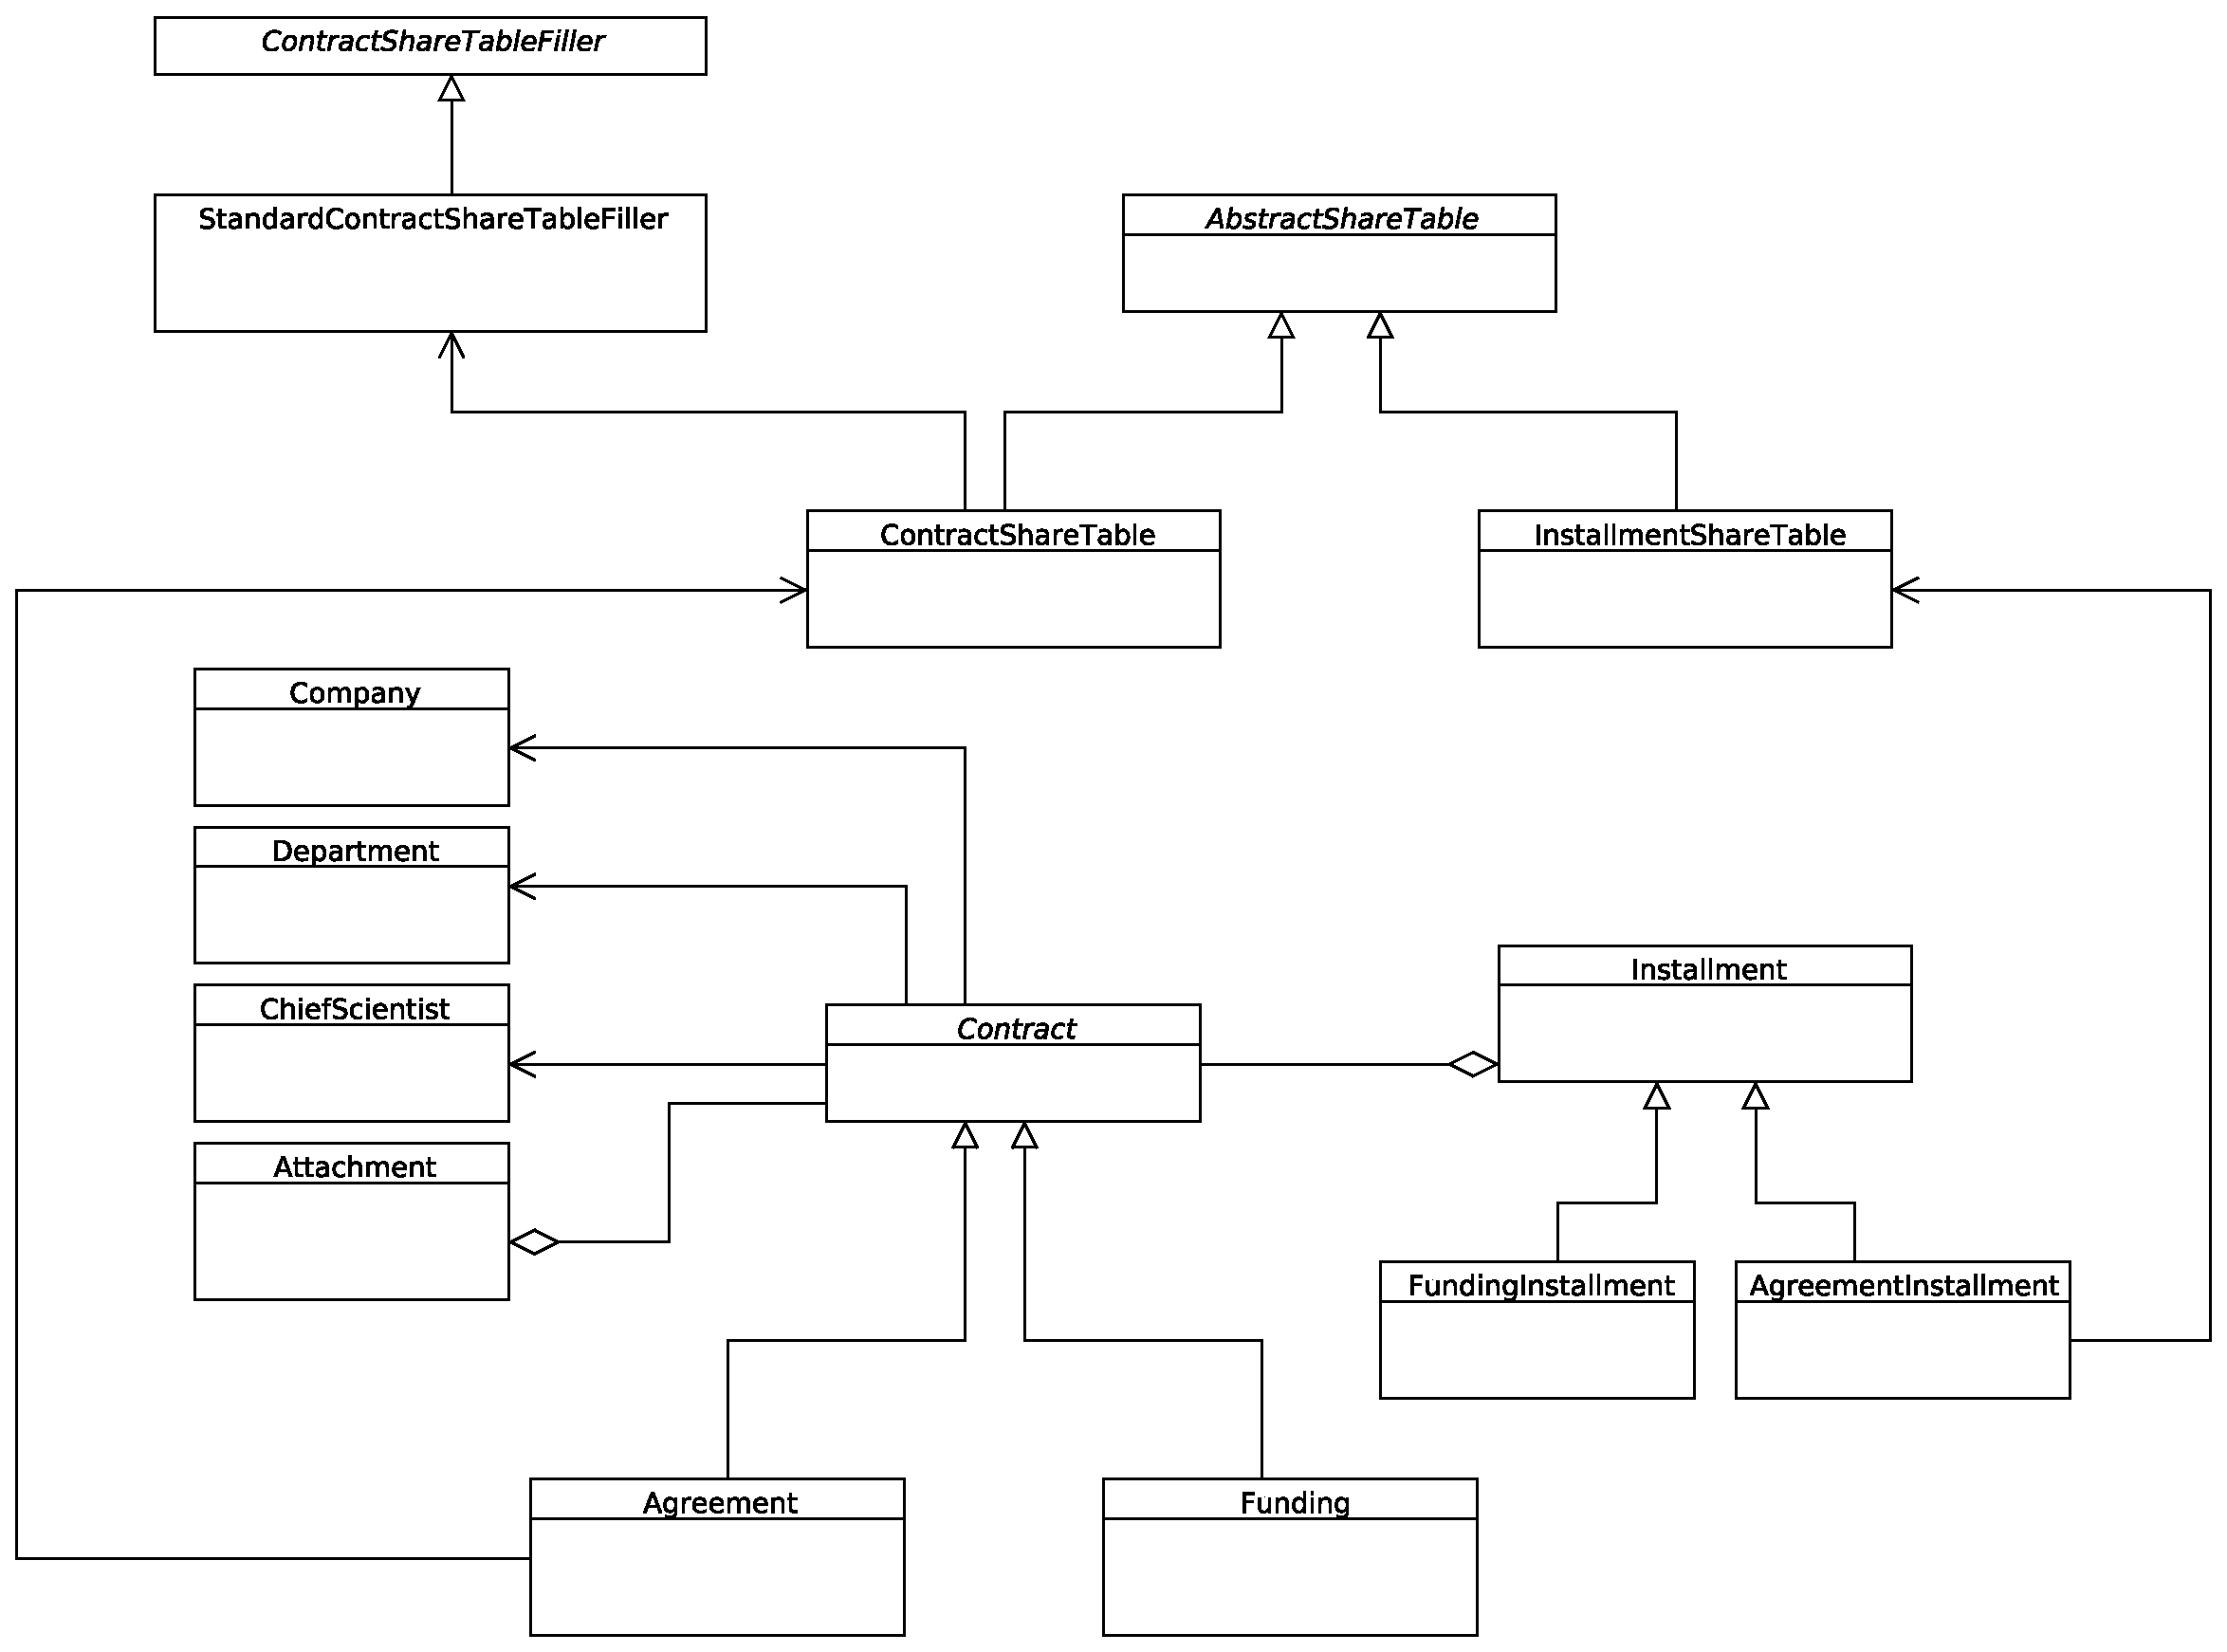
\includegraphics[width=1\textwidth]{images/modello_business.eps}
\end{figure}

\subsection{Modello degli utenti}

\begin{figure}[h]
	\centering
	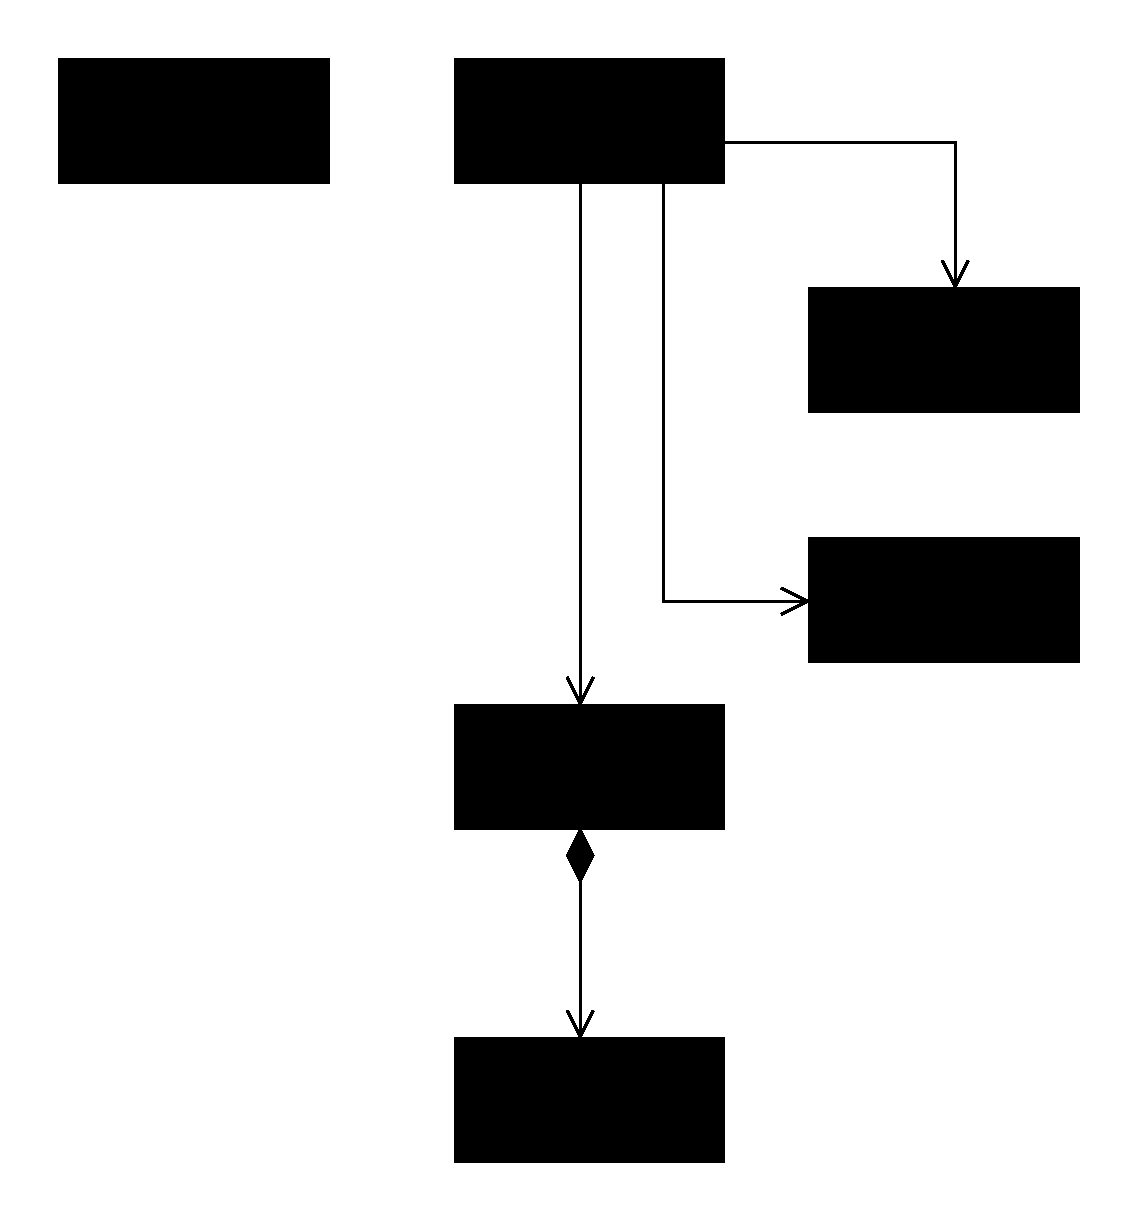
\includegraphics[width=0.6\textwidth]{user_model.eps}
	\caption{Modello degli utenti}
	\label{user_model}
\end{figure}

In figura \ref{user_model} è mostrato il modello degli utenti. \\
La classe centrale di tale modello è \texttt{User}, che rappresenta un generico utente dell'applicazione. I tipi di utente sono distinti tramite l'enum \texttt{Role}, che può avere quattro valori:

\begin{itemize}
\item \texttt{ADMIN} (\textsl{Amministratore}). Rappresenta, appunto, l'amministratore del sistema. È l'unico che può aggiungere altri utenti di tipo Operatore o Docente. Non è afferente ad alcun dipartimento.
\item \texttt{OPERATOR} (\textsl{Operatore}). Un Operatore gestisce le convenzioni del dipartimento a cui afferisce.
\item \texttt{PROFESSOR} \textsl{Docente}. Il Docente può consultare le proprie convenzioni e, se richiesto, allegare documenti alle stesse.
\item \texttt{GUEST}. Rappresenta l'utente non ancora loggato. Non possiede alcun permesso.
\end{itemize}

Le operazioni che un utente può svolgere sono regolate tramite un sistema di permessi, i quali sono rappresentati dalla enum \texttt{Permission}: ad ogni \texttt{Role} è associata una lista di \texttt{Permission}. Per maggiori dettagli riguardo la sicurezza, si rimanda al capitolo \ref{delta}.\\

Un utente ha quindi un attributo che ne identifica il ruolo. Vi sono poi degli attributi che lo caratterizzano (come ad esempio l'indirizzo e-mail) ed infine un attributo di tipo \texttt{Encryptor}. \\
La classe \texttt{Encryptor} racchiude metodi per gestire le diverse codifiche delle password, in modo da poter utilizzare stringhe codificate in maniera differente e rendere indipendente la codifica utilizzata dall'applicazione 
con quella che adopera il servizio esterno che fornisce le credenziali di Ateneo. Attualmente sono supportate due tipi di codifica: MD5 (la più utilizzata dal sistema di Ateneo) e 
SHA (adoperata anch'essa dal sistema di Ateneo, anche se in misura minore;). SHA è la codifica di default dell'applicazione).\\
\\

Parallela alla classe \texttt{User} vi è la classe \texttt{Principal}, che rappresenta l'utente dell'applicazione attualmente loggato. 
La differenza fra queste è sottile: le due classi infatti, rappresentano due aspetti diversi dell'utente: la prima modella l'utente all'interno dell'applicazione, la seconda, invece, serve per gestire la navigazione dell'utente. La classe \texttt{Principal} ha quindi due caratteristiche principali:
\begin{itemize}
\item è disaccoppiata dall'implementazione del modello: gli attributi del \texttt{Principal} sono di tipo stringa e ciò consente di cambiare l'implementazione sottostante indipendentemente dal \texttt{Principal}
\item è sicura, perché non contiene proprietà sensibili dell'utente (come ad esempio la password).
\end{itemize}




\section{Casi d'uso}
Di seguito si elencano i casi d'uso per ciascun tipo di utente che interagisce col sistema. 
\begin{enumerate}

\item \textbf{Utente generico}\\
Si racchiudono nella figura dell'Utente generico i casi d'uso che sono comuni a tutti gli altri tipi di utenti. Tali casi d'uso sono riportati in figura \ref{use_case_diag_generic}

\begin{figure}[h]
  \caption{Diagramma dei casi d'uso dell'Utente generico}
  \label{use_case_diag_generic}
  \centering
    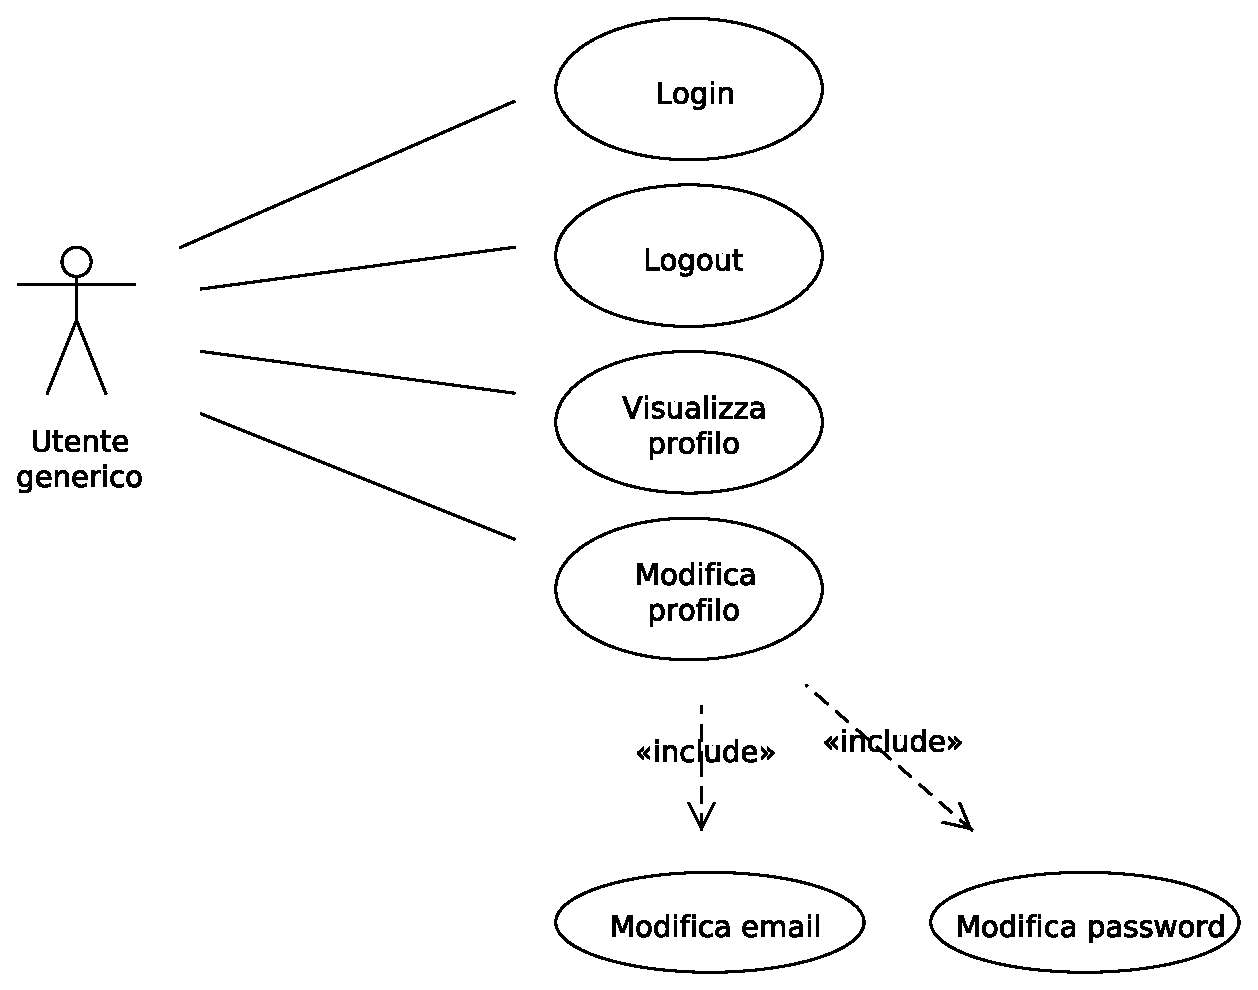
\includegraphics[width=0.7\textwidth]{images/casi_uso_utente_generico.eps}
\end{figure}

\begin{enumerate}

 \item Login\\ \label{UC_login}
    Percorso base:
    l'Utente Generico, dopo aver raggiunto l'indirizzo web dell'applicativo, inserisce il proprio numero di matricola e password, quindi clicca sul pulsante ``Login". Viene visualizzata la pagina iniziale.\\
    Percorso alternativo:
    l' Utente Generico inserisce i propri dati personali ma commette un errore, quindi clicca su ``Login". Viene visualizzato un messaggio nel quale si avvisa l'utente dell'errore commesso.
    
 \item Visualizzazione del profilo\\ \label{UC_view_profile}
    Dopo aver effettuato il login , l'Utente Generico clicca sul pulsante ``Profilo" nella toolbar in alto; si presenta una schermata contente i dati personali dell'Utente.
 \item Modifica dell'indirizzo e-mail\\ \label{UC_edit_email}
  Percorso base:
  dopo aver effettuato il login , l'Utente Generico clicca sul pulsante ``Profilo" nella toolbar in alto; si presenta una schermata contente i dati personali dell'Utente.
  L'Utente cambia il proprio indirizzo e-mail. Una volta effettuate le modifiche desiderate l'Utente clicca su ``Salva". Le modifiche vengono salvate e viene visualizzata la schermata precedente.\\
  
  Percorso alternativo:
  l'Utente inserisce una e-mail non valida. L'Utente è avvertito dell'errore con un messaggio ed è invitato a riprovare.
\end{enumerate}



\item \textbf{Operatore}\\
Una rappresentazione grafica dei casi d'uso dell'Operatore è disponibile in figura \ref{use_case_diag_operator}
\begin{figure}[h]
  \caption{Diagramma dei casi d'uso dell'Operatore}
  \label{use_case_diag_operator}
  \centering
    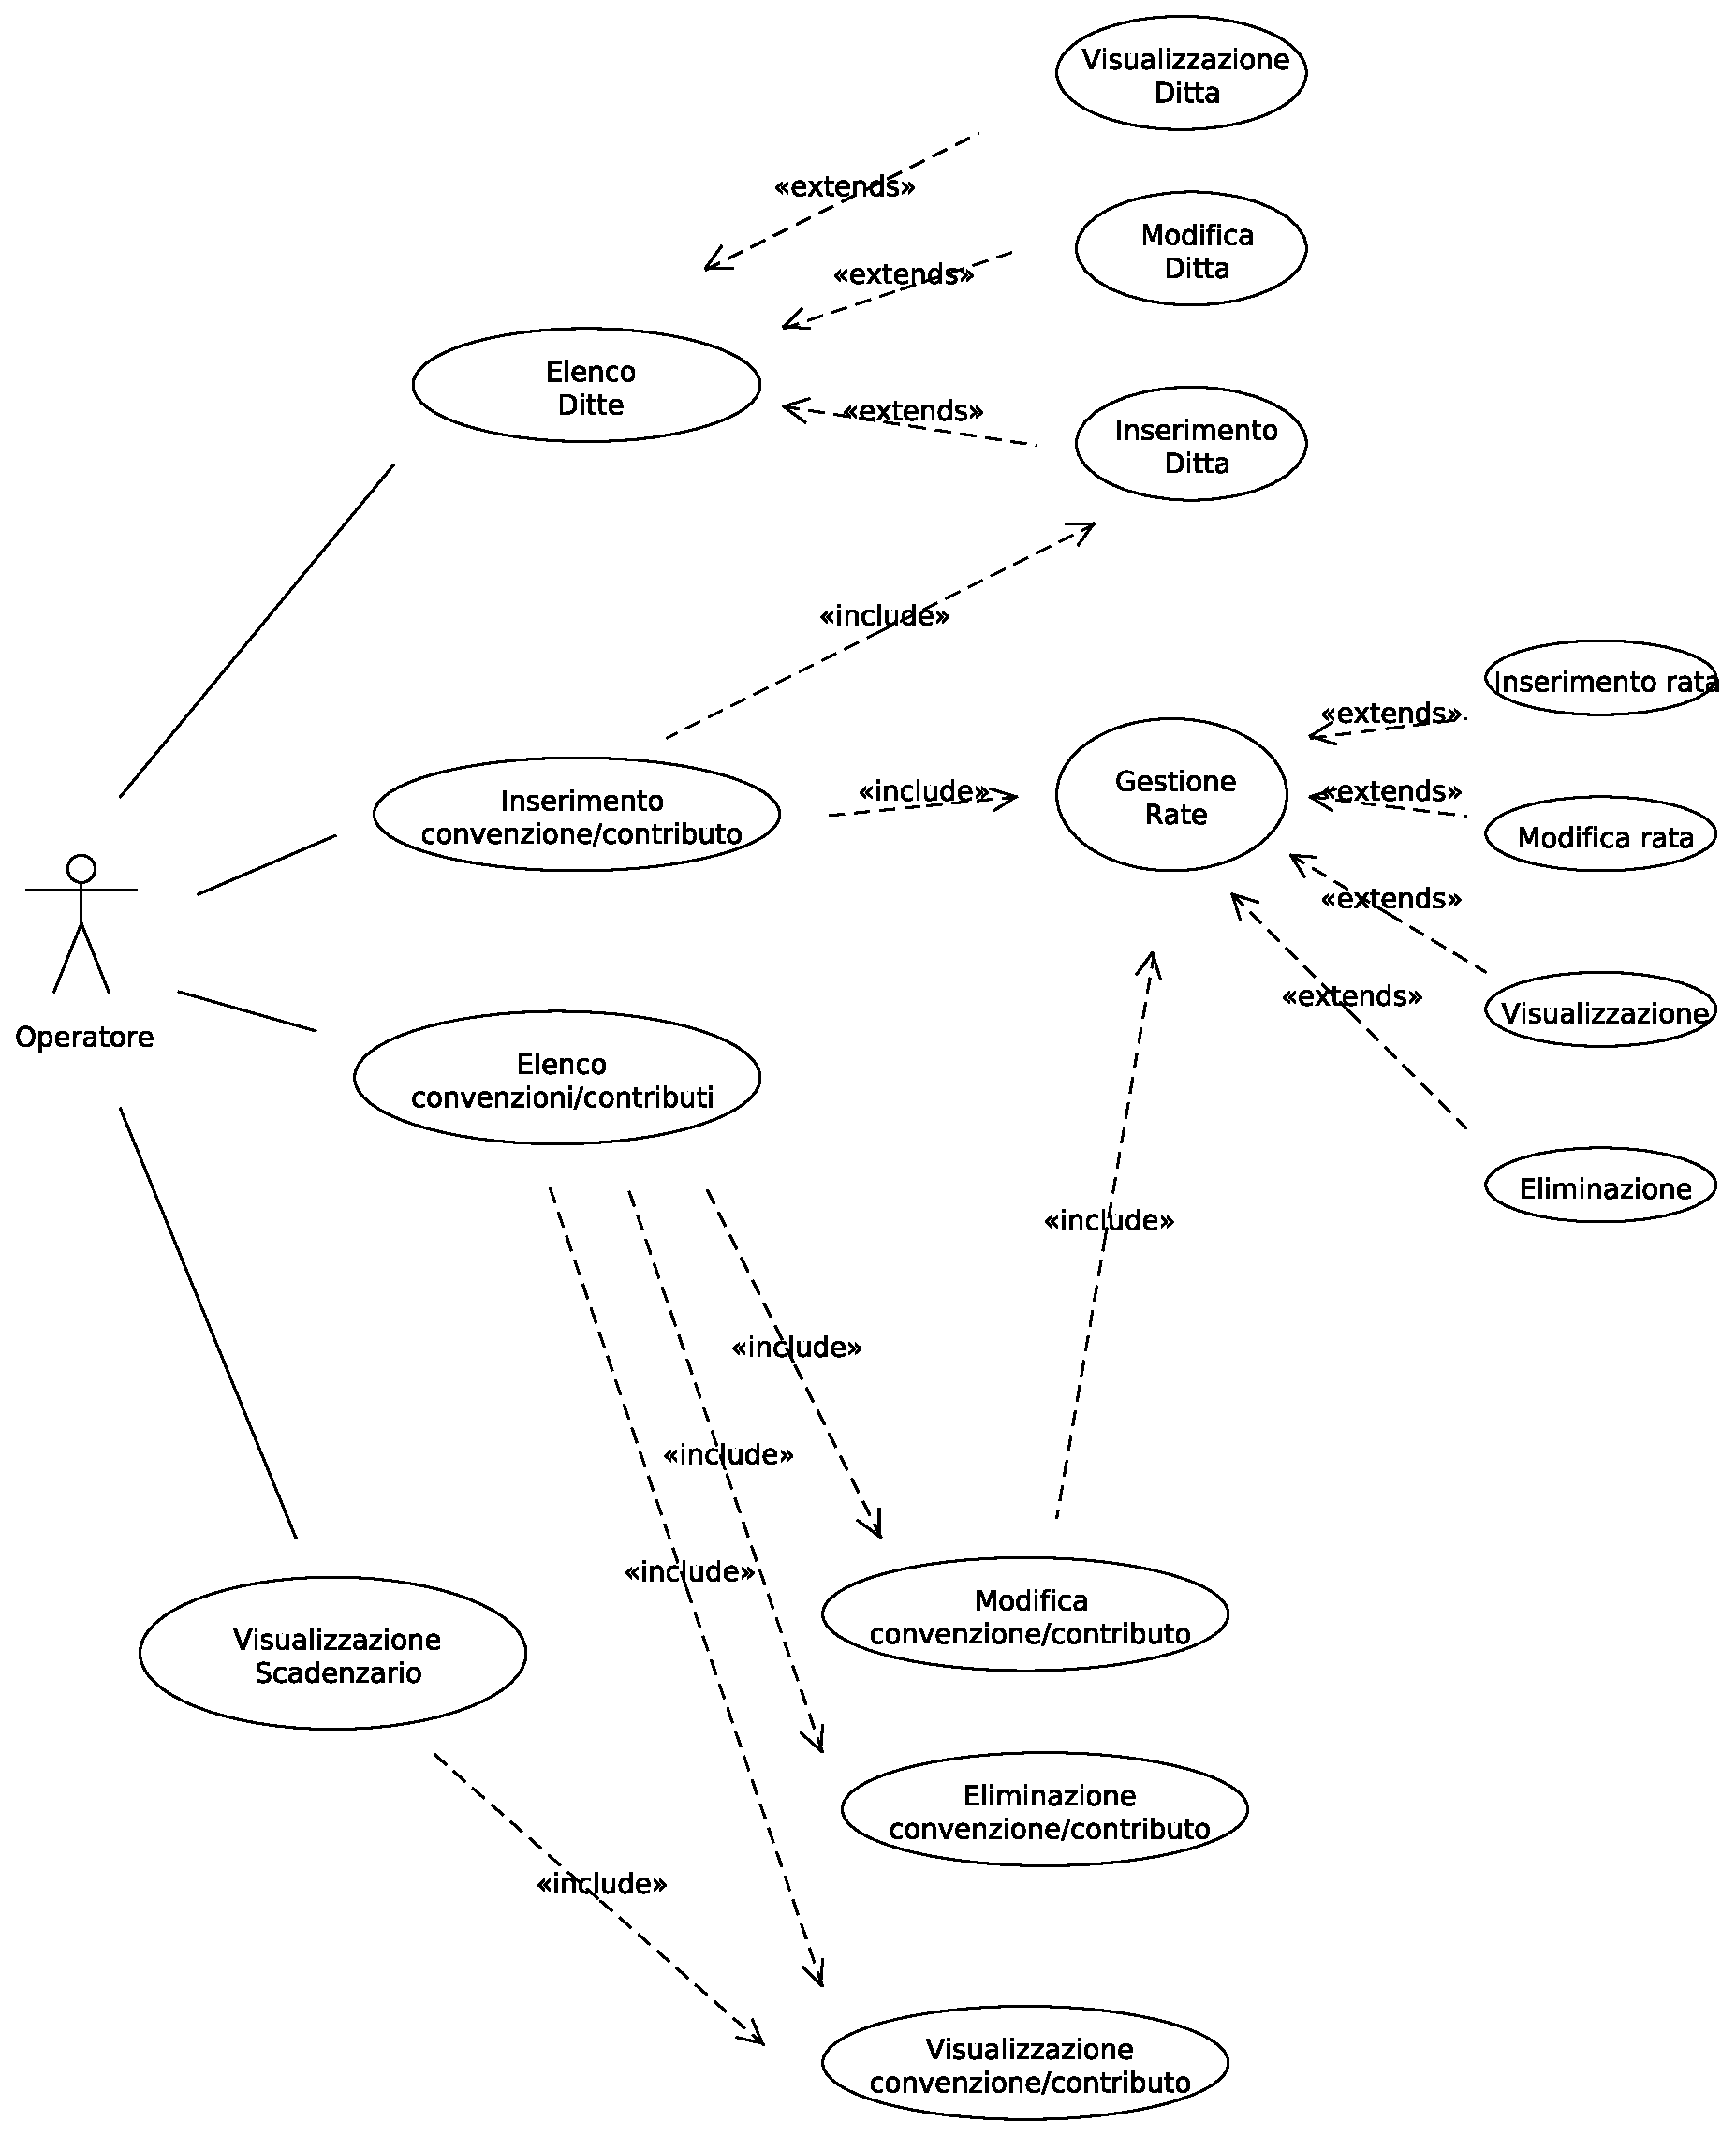
\includegraphics[width=1\textwidth]{images/casi_uso_operatore.eps}
\end{figure}

\begin{enumerate}
  \item Inserimento di una nuova Convenzione/Contributo\\ \label{UC_new_contract}
  
  Percorso base:
  l'Operatore, una volta effettuato il login, clicca su ``Crea una convenzione/contributo"; viene visualizzata una schermata suddivisa in varie schede,
  ognuna corrispondente ad un passo della procedura. E' possibile passare da una vista all'altra mediante i pulsanti ``Avanti" e ``Indietro". I passi sono:
  \begin{enumerate}
    \item Inserimento dei dati della convenzione/contributo\\
      
      In questa scheda sono elencati tutti i campi necessari per la definizione di una convenzione/contributo, 
      che l'Operatore deve compilare. Tali campi sono:
      \begin{itemize}
	\item Il titolo
	\item Il titolo riassuntivo
	\item Il numero di protocollo
	\item L'UAR
	\item La tipologia
	\item Il responsabile scientifico\\
	  Per selezionare un responsabile scientifico è possibile usare l'apposito menù a tendina o, in alternativa, qualora la persona cercata non sia nell'elenco, aggiungerla cliccando sul pulsante ``Aggiungi".
	\item Il referente
	\item La ditta\\
	  Per selezionare una ditta si può usare l'apposito menù a tendina o, se la ditta cercata non fosse presente nell'elenco, aggiungerne una nuova cliccando sul pulsante ``Aggiungi".Per ulteriori dettagli si rimanda \ref{UC_new_company}.
	\item Il nome del progetto CIA
	\item Il Repertorio
	\item Il totale imponibile
	\item L'Iva
	\item La data di approvazione
	\item La data di inizio
	\item La data di scadenza
      \end{itemize}
      
      Nota : i campi riguardanti l'Iva non sono presenti nel caso del contributo.
      
    \item Inserimento della tabella di ripartizione\\
     
      Questa scheda contiene le voci della tabella di ripartizione. L'Operatore può modificare alcuni valori percentuali 
      in base ai quali dividere l'importo totale. Le voci non modificabili sono calcolate in relazione ai campi modificabili facendo riferimento alle norme di ateneo. Le voci modificabili sono:
      \begin{itemize}
	\item Personale: stabilisce la quota destinata al personale; è l'unico campo principale che l'operatore può modificare e in base al quale vengono calcolati gli altri.
	\item Missioni, Materiale di consumo, etc. sono sotto-campi di Beni e Servizi e servono per meglio specificare come verrà ripartita la quota destinata a ``Beni e Servizi".
      \end{itemize}
      
      Nota : questa scheda è assente nel caso del contributo, non essendo prevista una ripartizione.
    \item Gestione delle rate\\
      
      Questo passo della procedura è facoltativo: viene data la possibilità all'operatore di inserire delle rate per la convenzione/contributo
      che sta creando. Una volta inserite una o più rate
      queste vengono visualizzate in una tabella e l'Operatore
      ha la possibilità di modificare, visualizzare o eliminare una rata cliccando sui tasti ``Modifica",``Visualizza" ed ``Elimina" che compaiono sulla sinistra, nella riga della tabella
       corrispondente alla rata in questione. Per i dettagli riguardo alle operazioni sulle rate si rimanda ai corrispettivi casi d'uso.

      
    \item Inserimento della documentazione relativa alla convenzione\\
	  
	  Questa scheda elenca i documenti allegati alla convenzione. L'Operatore può aggiungere o eliminare un documento 
	  cliccando sugli appositi tasti. Premendo il tasto ``Salva" la convenzione viene salvata e la procedura termina. Si ritorna alla schermata precedente.
  \end{enumerate}
		 
  Percorso alternativo 1:
  Durante uno qualsiasi dei passi, l'Operatore  clicca sul tasto ``Annulla", che comporta, a seguito di una conferma, il ritorno alla schermata precedente
  senza che la convenzione/contributo venga inserita o i cambiamenti effettuati salvati.
  
  Percorso alternativo 2:
  l'Operatore clicca sul tasto ``Salva" senza aver compilato alcuni dei campi obbligatori, o avendo inserito dei valori non consentiti; viene visualizzato un messaggio di errore 
  e il documento non viene salvato. La schermata non viene cambiata, dando la possibilità all'Operatore di procedere alla correzione.
     
  \item Visualizzazione delle convenzioni/contributi\\ \label{UC_view_contract_list}

  Percorso base:
  l'Operatore clicca su ``Visualizza contratti"; viene mostrata una lista delle convenzioni/contributi correntemente stipulate in 
  riferimento al dipartimento di afferenza dell'Operatore, con opportuni filtri 
  per agevolare la ricerca (tra cui un filtro per data di scadenza) e ordinabili per data.
  L'Operatore può selezionare una convenzione e, mediante gli appositi pulsanti che appaiono sulla sinistra, modificare, visualizzare o eliminare una convenzione. Per i dettagli si rimanda casi d'uso relativi a tali operazioni.\\	

  Percorso alternativo:
  L'Operatore clicca sul tasto ``Home", si torna alla pagina iniziale.
 
  \item Modifica di una convenzione/contributo\\ \label{UC_edit_contract}
  
  Percorso base:
  l'Operatore a partire dalla schermata ``Visualizzazione Contratti" clicca sul pulsante ``Modifica" che appare sulla sinistra nella riga 
  della tabella corrispondente alla convenzione/contributo desiderata. Viene visualizzata una schermata suddivisa in schede analoga a quella
  descritta nel caso della ``Creazione di una convenzione/contributo", con la differenza che in questo caso è possibile spostarsi da una scheda all'altra
  cliccando sulla scheda stessa. Inoltre è presente la scheda aggiuntiva ``Riepilogo" che contiene alcune informazioni di riepilogo come il residuo
  totale della convenzione/contributo o il totale fatturato.
  L'Operatore effettua i cambiamenti desiderati quindi clicca sul pulsante ``Salva"; i dati vengono salvati e si ritorna all'elenco delle convenzioni/contributi\\

  Percorso alternativo 1:
  l'Operatore clicca sul tasto \textquotedblleft Annulla" da qualsiasi scheda;  si torna alla schermata \textquotedblleft Visualizzazione Contratti" senza salvare le modifiche effettuate.\\
  
  Percorso alternativo 2:
  l'Operatore clicca su \textquotedblleft Salva" ma alcuni valori immessi non sono corretti, viene visualizzato un messaggio di errore e non si torna alla schermata \textquotedblleft Visualizzazione delle
  convenzioni/contributi" dando la possibilità all'Operatore di correggere gli errori commessi prima di salvare nuovamente.
  
  \item Visualizzazione di una convenzione/contributo\\ \label{UC_view_contract}
 
  Del tutto analogo a ``Modifica di una convenzione/contributo" con la differenza che in questo caso non è possibile modificare i dati della
  convenzione/contributo.
  
  \item Eliminazione di una convenzione/contributo\\ \label{UC_delete_contract}
  
  Percorso base:
  l'Operatore a partire dalla schermata ``Visualizzazione Contratti" clicca sul pulsante ``Elimina" che appare sulla sinistra nella riga 
  della tabella corrispondente alla convenzione/contributo desiderata. Appare una finestra di dialogo che chiede di confermare l'operazione. L'Operatore clicca sul pulsante ``Sì", la convenzione/contributo viene eliminato e si
  ritorna alla schermata precedente.
  
  Percorso alternativo:
  l'Operatore, dopo aver cliccato su ``Elimina", essendosi accorto di aver commesso un errore, clicca sul pulsante ``No". La convenzione/contributo non viene eliminata e si ritorna alla schermata precedente.
  
  
  
\item Inserimento di una rata\\ \label{UC_new_installment}
Percorso base:
l'Operatore può inserire una rata sia in fase di creazione della convenzione/contributo sia in fase di modifica; in entrambi i casi dopo aver raggiunto
la scheda ``Rate" l'Operatore clicca sul pulsante ``Aggiungi una rata".  
Viene visualizzata una finestra di dialogo suddivisa in varie schede,
ognuna corrispondente ad un passo della procedura. E' possibile passare da una scheda all'altra mediante i pulsanti \textquotedblleft Avanti" e \textquotedblleft Indietro". I passi sono:
\begin{enumerate}
  \item Inserimento dei dati della rata\\
  
  L'operatore inserisce i seguenti campi
    \begin{itemize}
    \item Importo
    \item Iva
    \item Data
    \item Numero Reversale
    \item Data Reversale
    \item Numero di Sospeso
    \item Numero di fatturato
    \item Data fatturata
    \item È stata pagata la fattura?
    \item Deve essere allegata la fattura?
    \item Note
    \end{itemize}
    
   Nota : i campi riguardanti l'Iva non sono presenti nel caso del contributo.

   
  \item Inserimento della tabella di ripartizione\\
  
  Il procedimento è del tutto analogo a quello descritto nel caso d'uso \textquotedblleft Inserimento della tabella di ripartizione" per l'inserimento di 
  una nuova convenzione/contributo. 
\end{enumerate}

L'Operatore clicca pulsante \textquotedblleft Salva".Le modifiche vengono salvate e si torna alla schermata precedente;

Percorso alternativo:
l'Operatore clicca sul pulsante ``Annulla", viene chiusa la finestra di dialogo senza che la rata sia stata inserita.

\item Modifica di una rata\\ \label{UC_edit_installment}

Percorso base:
l'Operatore accede alla schermata ``Visualizzazione contratti" cliccando sul pulsante apposito nella pagina iniziale, quindi seleziona la convenzione/contributo alla quale la rata appartiene e clicca sul pulsante ``Modifica" che compare
all'interno della riga selezionata. Viene così visualizzata la schermata ``Modifica di una convenzione/contributo"; l'Operatore raggiunge la scheda ``rate" e clicca sul pulsante ``Modifica" che compare selezionando la riga della tabella
corrispondente alla rata desiderata. Viene visualizzata una finestra di dialogo composta di varie schede analoghe a quelle descritte nel caso dell'inserimento. E' possibile passare da una scheda all'altra cliccando su di esse.
Dopo avere effettuato le modifiche richieste l'Operatore clicca sul pulsante ``Salva", la convenzione/contributo viene aggiornata e viene visualizzata la schermata precedente.

Percorso alternativo:
l'Operatore clicca sul pulsante ``Annulla", le modifiche vengono scartate e si torna alla schermata precedente.

\item Visualizzazione di una rata \label{UC_view_installment}

Una volta raggiunta la scheda ``rate" relativa alla convenzione/contributo di interesse l'Operatore, dopo aver selezionato la rata desiderata, clicca sul pulsante ``Visualizza". Viene presentata una finestra di dialogo analoga a quella descritta nel caso della modifica 
con la differenza che i campi non sono modificabili. E' possibile tornare alla schermata precedente cliccando sul pulsante ``Indietro".

\item Eliminazione di una rata\\ \label{UC_delete_installment}

Raggiunta la scheda ``rate" relativa alla convenzione/contributo di interesse, l'Operatore, dopo aver selezionato la rata di interesse, clicca sul pulsante ``Elimina'; appare una finestra di dialogo che chiede di confermare
l'eliminazione, l'Operatore clicca "Sì"la rata viene eliminata e si torna alla schermata precedente.

\item Inserimento di una Ditta\\ \label{UC_new_company}
Percorso base:
l'Operatore clicca su ``Visualizza elenco Ditte" dalla pagina iniziale; viene visualizzata una schermata contenente un elenco delle ditte inserite. L'Operatore clicca sul pulsante ``Aggiungi" in basso a sinistra. Viene visualizzata
una finestra di dialogo contente i seguenti campi obbligatori:
\begin{itemize}
 \item Denominazione
 \item Ragione sociale
 \item Sede Legale
 \item Codice fiscale
 \item Partita IVA
\end{itemize}
l'Operatore dopo aver riempito i campi clicca su ``Salva", la nuova ditta viene salvata e si ritorna alla schermata precedente.

Percorso alternativo:
l'Operatore clicca su ``Salva" senza aver riempito tutti i campi obbligatori, viene visualizzato un messaggio di errore che invita l'utente inserire tali campi.

Percorso alternativo 2:
l'Operatore clicca su ``Salva" avendo inserito un codice fiscale di una ditta già inserita. Viene visualizzato un opportuno messaggio di errore.

Percorso alternativo 3:
si può inserire una ditta anche in fase di creazione di una convenzione/contributo cliccando sul pulsante ``Aggiungi" accanto al campo ``ditta" nella scheda ``Dati generali".

\item Modifica di una Ditta\\ \label{UC_edit_company}

Percorso base:
l'Operatore clicca su ``Visualizza elenco Ditte" dalla pagina iniziale; viene visualizzata una schermata contenente un elenco delle ditte inserite. L'Operatore dopo aver posizionato il cursore sulla riga dell'elenco
corrispondente alla ditta di interesse clicca sul pulsante ``Modifica"che appare a sinistra sulla riga selezionata. Viene visualizzata
una finestra di dialogo analoga a quella dell'inserimento.

l'Operatore dopo aver modificato i campi desiderati clicca su ``Salva", la  ditta viene salvata e si ritorna alla schermata precedente.

Percorso alternativo:
l'Operatore clicca su ``Salva" senza aver riempito tutti i campi obbligatori, viene visualizzato un messaggio di errore che invita l'utente a inserire tali campi.

Percorso alternativo 2:
l'Operatore clicca su ``Salva" avendo inserito un codice fiscale di una ditta già inserita. Viene visualizzato un opportuno messaggio di errore.

\item Visualizzazione di una Ditta\\ \label{UC_view_company}
  Percorso base:
  l'Operatore raggiunge l'elenco delle ditte quindi clicca sul pulsante ``Visualizza ditta" che compare sulla sinistra selezionando la riga dell'elenco corrispondente alla ditta desiderata.

\item Visualizzazione dell'elenco delle ditte\\ \label{UC_view_company_list}
  Percorso base:
  l'Operatore dalla pagina iniziale clicca sul pulsante ``Visualizza elenco ditte". Viene presentata una schermata contente un elenco di ditte filtrabili per nome attraverso l'apposito filtro di ricerca.
  
\item Visualizzazione dello Scadenzario\\ \label{UC_view_deadlines}
  Percorso base:
  l'Operatore dalla pagina iniziale clicca sul pulsante ``Visualizza scadenzario", Viene presentata una schermata contente un elenco di contratti che hanno delle rate con scadenze attive. E' possibile filtrare i risultati in base a vari
  criteri di ricerca. Selezionando una convenzione/contributo e cliccando sul pulsante ``Visualizza" che compare sulla destra è possibile visualizzare una convenzione/contributo, per i dettagli su questa operazione si rimanda a \ref{UC_view_contract}

\end{enumerate}

 
\item \textbf{Docente}\\
I casi d'uso del Docente sono rappresentati in figura \ref{use_case_diag_teacher}
\begin{figure}[h]
  \caption{Diagramma dei casi d'uso del Docente}
  \label{use_case_diag_teacher}
  \centering
    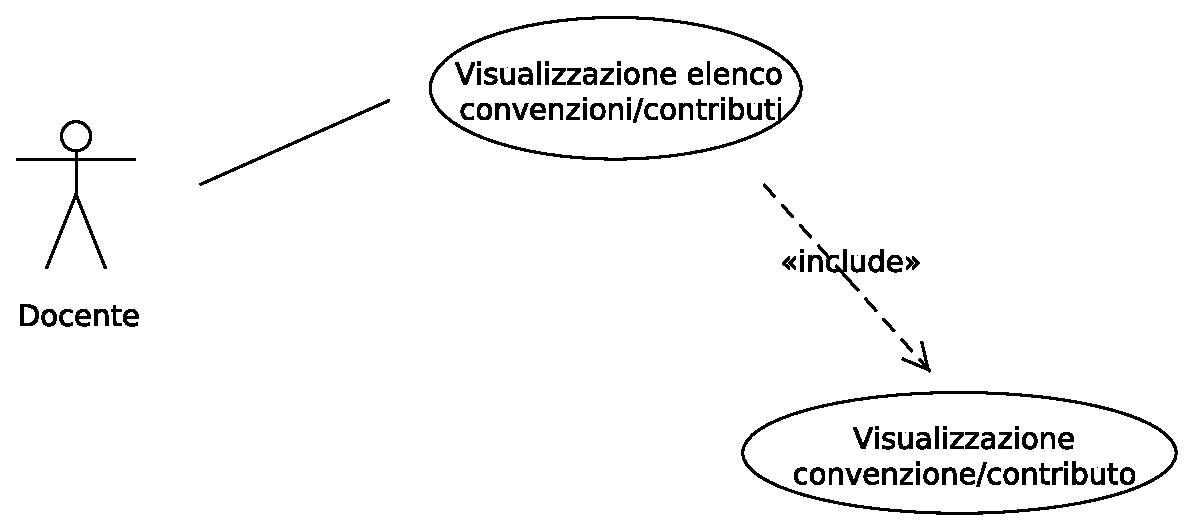
\includegraphics[width=0.8\textwidth]{images/casi_uso_docente.eps}
\end{figure}

\begin{enumerate}
 
 \item Visualizzazione dell'elenco delle convenzioni/contributi di cui il docente è responsabile scientifico\\ \label{UC_view_own_contract_list}
 
 Il docente, dopo aver effettuato il login, può cliccare sul pulsante ``Visualizzazione della lista delle convenzioni/contributi"; la schermata
 che viene visualizzata contiene una tabella che elenca le convenzioni/contributi del docente. E' possibile filtrare le convenzioni/contributi
 secondo vari criteri(data, tipo, scadenze più vicine, ...).Inoltre è possibile visualizzare i dettagli di una convenzione/contributo cliccando sul
 pulsante ``Visualizza" che appare posizionando il puntatore su una riga della tabella.
 
 \item Visualizzazione di una convenzione/contributo di cui il docente è responsabile scientifico\\ \label{UC_view_own_contract}
 
 Il docente dalla schermata ``Visualizzazione delle convenzioni/contributi" può cliccare sul pulsante ``Visualizza" relativo ad una convenzione/contributo; compare una schermata suddivisa in schede analoga a quella della modifica/creazione
 della convenzione. Il docente può navigare fra le schede cliccandoci sopra. Non è permessa nessuna modifica ai dati della convenzione/contributo, tuttavia il docente può gestire gli allegati dalla scheda ``Allegati", per i dettagli
 si rimanda a \ref{UC_manage_attachments}. Cliccando su ``Salva"
 gli allegati inseriti dal docente vengono memorizzati, al contrario cliccando su ``Indietro" le modifiche vegono scartate.
 
 \item Gestione allegati\\ \label{UC_manage_attachments}
  
 Percorso base:
 il Docente raggiunge la scheda ``Allegati" di una convenzione/contributo quindi:
  \begin{itemize}
   \item clicca su ``Aggiungi", viene presentata una finestra di dialogo che consente di selezionare un file da inserire come allegato.
   \item clicca sul pulsante ``Download" che compare sulla destra selezionando una riga della tabella degli allegati. Il file corrispondente a tale riga viene scaricato sul computer dell'utente.
   \item clicca sul pulsante ``Rimuovi" che compare sulla destra selezionando una riga della tabella degli allegati. Il file corrispondente viene rimosso dagli allegati della convenzione/contributo
  \end{itemize}
 il docente clicca quindi su ``Salva", le modifiche vengono apportate e si ritorna alla schermata precedente.
 
 Percorso alternativo:
 il Docente, dopo aver effettuato alcune modifiche clicca su ``Indietro", le modifiche non vengono salvate e si ritorna alla schermata precedente.

 
\end{enumerate}



\item \textbf{Amministratore}\\
Una rappresentazione dei casi d'uso dell'Amministratore è disponibile in figura \ref{use_case_diag_admin}
\begin{figure}[h]
  \caption{Diagramma dei casi d'uso dell'Amministratore}
  \label{use_case_diag_admin}
  \centering
    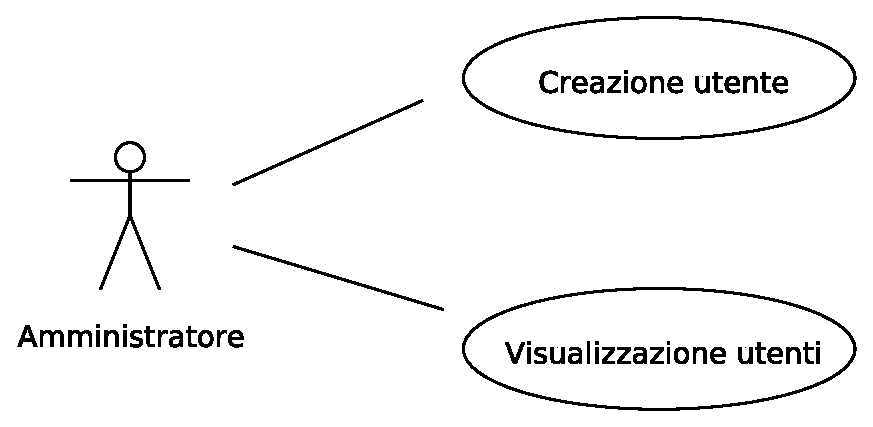
\includegraphics[width=0.6\textwidth]{casi_uso_amministratore.eps}
\end{figure}


\begin{enumerate}
 \item Inserimento di un nuovo utente\\ \label{UC_new_user}
 
 
 Percorso base:
 l'Amministratore, dopo aver effettuato il login, clicca sul pulsante ``Crea nuovo utente"; viene visualizzata una schermata che permette
 di inserire i dati dell'utente:
 \begin{itemize}
  \item Nome
  \item Cognome
  \item Matricola
  \item E-mail
  \item	Password\\
    In realtà i campi che l'Amministratore deve riempire sono due: un campo password ed un campo di verifica che deve corrispondere col precedente.
  \item Ruolo\\
    L'Amministratore può scegliere il ruolo dal rispettivo menù a tendina, i ruoli disponibili sono Operatore, Amministratore, Docente.
 \end{itemize}
 
 Una volta completato l'inserimento, l'Amministratore clicca sul pulsante ``Salva", il nuovo utente viene registrato nel sistema. 

 Percorso alternativo 1:
 l'Amministratore inserisce solo il campo matricola e quindi clicca il pulsante ``Importa Utente da LDAP". I rimanenti campi, se la matricola è valida,
 vengono automaticamente importati dal servizio LDAP offerto da SIAF. L'Amministratore conclude la procedura cliccando sul pulsante ``Salva"
 
 Percorso alternativo 2:
 l'Amministratore in qualunque momento della procedura clicca sul pulsante ``Annulla"; viene presentata a video la schermata precedente,
 nessun utente viene aggiunto al sistema.
 
 \item Visualizzazione della lista degli utenti \label{UC_view_user_list}
  L'Amministratore, una volta effettuato il login, clicca sul pulsante ``Visualizza utenti"; viene presentata una schermata contenente una lista  degli
  utenti inseriti nel sistema. L'Amministratore clicca sul pulsante ``Indietro" per tornare alla pagina iniziale.
\end{enumerate}

\item \textbf{Tempo}\\
I casi d'uso del Tempo sono rappresentati in figura \ref{use_case_diag_teacher}
\begin{figure}[h]
  \caption{Diagramma dei casi d'uso del Tempo}
  \label{use_case_diag_time}
  \centering
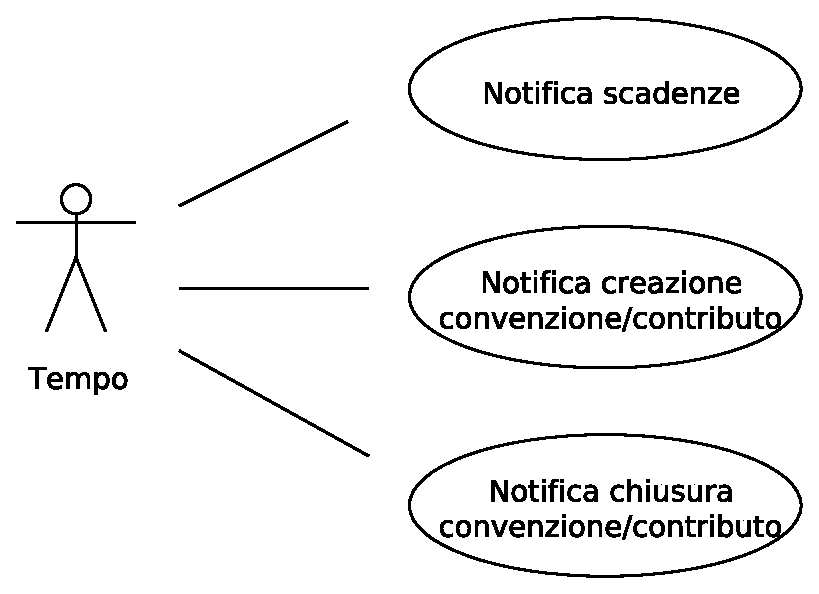
\includegraphics[width = 0.5\textwidth]{images/casi_uso_tempo.eps}
\end{figure}
\begin{enumerate}
 \item Notifica delle scadenze\\ \label{UC_notify_deadlines}
 
    Ad intervalli periodici stabiliti, i docenti che hanno convenzioni/contributi attive con rate in scadenza ravvicinata, vengono avvertiti tramite posta elettronica.
  
 
 \item Notifica della creazione di una nuova convenzione/contributo\\ \label{UC_notify_new_contract}
 
    Al momento del completamento della creazione di una nuova convenzione/contributo viene inviata una e-mail all'indirizzo di posta elettronico del responsabile scientifico indicato per la convenzione/contributo. Tale e-mail contiene
    le informazioni principali che caratterizzano la convenzione/contributo.
  
  
 \item Notifica della chiusura di una convenzione/contributo\\ \label{UC_notify_closed_contract}
 
    Al momento della chiusura di una convenzione/contributo (ovvero quando il fatturato è pari all'importo totale) viene inviata una e-mail all'indirizzo di posta elettronico del responsabile scientifico che notifica la chiusura della
    convenzione/contributo riportando alcuni dati di questa.
\end{enumerate}


\end{enumerate}


\chapter{Tecnologie}
L'applicativo sviluppato si basa sulla piattaforma \textsl{Java EE}, in particolare sfrutta i moduli \textsl{JPA} per la persistenza e \textsl{CDI} per la gestione del ciclo di vita dei bean e per l'iniezione di dipendenza. L'interfaccia grafica
invece è stata scritta usando il framework \textsl{JSF} mentre per quanto riguarda la sicurezza si è utilizzato \textsl{DeltaSpike}. Come application server è invece stato scelto \textsl{JBoss AS 7}. Di seguito una descrizione di ciascuno
di questi framework e, infine, di altre librerie usate per particolari contesti.
\label{tecnologie}
\section{JPA}
\label{jpa}
\subsection{Introduzione}
Le applicazioni di tipo Enterprise necessitano di raccogliere e persistere grandi quantità di informazioni, la soluzione che più si è affermata per risolvere questo problema è il database relazionale. Nell'ambiente Enterprise
, in particolare per la piattaforma Java, si è sentita l'esigenza di soluzioni che permettessero l'integrazione della piattaforma Java con database di tipo relazionale, in modo naturale. 

\subsection{Mapping fra modello Relazione e a Oggetti}
In un modello a oggetti,come il modello di dominio di un applicativo Java, le entità che popolano il modello sono Classi. Le relazioni fra le classi del modello sono espresse tramite riferimenti, gli attributi di una classe.
Nel modello relazionale invece le entità sono chiamate Relazioni e sono collegate fra loro mediante il concetto di chiave. Effettuare un mapping fra i due modelli significa quindi avere un modo per trasferire i concetti da un modello
all'altro in modo da ridurre le distanze fra i due modelli. In particolare una soluzione per il mapping dovrebbe avere le seguenti caratteristiche:

\begin{itemize}
 \item le applicazioni dovrebbero essere scritte e pensate secondo il modello di dominio e senza avere legami col modello relazione del database; dovrebbe essere possibile recuperare informazioni dal database senza dover scrivere espressioni
 che coinvolgano tabelle o chiavi primarie tipiche di un database.
 \item la soluzione dovrebbe essere non intrusiva: sebbene sia impensabile di realizzare una soluzione che renda la persistenza completamente trasparente, si può richiedere che la persistenza non ``invada'' il modello di dominio.
  In concreto le classi del dominio non devono essere obbligate ad implementare interfacce o estendere particolari classi per poter essere rese persistenti.
  \item dovrebbe essere possibile integrarsi con database preesistenti
\end{itemize}


\subsection{Struttura e caratteristiche di JPA}
Nel tempo sono state sviluppate e proposte varie soluzioni, a partire da ODBC passando per JDBC e EJB fino ad arrivare a \textsl{JPA}.
JPA (Java Persistence API) è una specifica per il mapping fra modello a oggetti e modello relazionale per applicazioni Java che, risolvendo i problemi degli standard precedenti, raggiunge
gli obiettivi sopra formulati. Esistono vari prodotti che implementano JPA fra cui \textsl{Hibernate} che è stato scelto come
implementazione per l'applicativo.\\
Di seguito si illustrano alcuni concetti e caratteristiche chiave della specifica, per ulteriori dettagli vedere \cite{jpa}.

\paragraph{Entity}
Un' unità che possegga una stato e che possa essere persistita viene detta Entità. Le classi Java possono essere facilmente trasformate in entità semplicemente annotando la classe stessa e alcuni dei suoi attributi, o alternativamente,
fornendo dei descrittori xml. L'unico
requisito che la classe deve rispettare è che deve possedere un costruttore senza parametri: questo serve affinché Hibernate (o qualsiasi altro provider) possa ricreare l'oggetto una volta interrogato il database per poi riempire i suoin campi.
Come si può notare, 
non è possibile rendere persistibile una classe in modo del tutto trasparente, ma di sicuro si può affermare che questo avvenga in modo non intrusivo. Allo stesso modo, sempre usando delle annotazioni o dei file di descrizione xml, 
è possibile mappare le relazioni che sussistono fra le entità del modello.

\paragraph{Entity Manager e Persistence Context}
Le Entità sono gestite da un Entity Manager. Un entity Manager è in grado di persistere un entità nonché di eliminarla o recuperarla dal database. Ogni Entity Manager è associato ad un Persistence Context. Un Persistence Context è un insieme di
istanze di entità. Una entità si dice ``managed'' se è contenuta in un Persistence Context. Se un Persistence Context, tramite un Entity Manager, partecipa ad una transazione lo stato delle entità ``managed'' contenuto in memoria
centrale viene salvato sul database. Le entità non ``managed'' sono chiamate ``detached'' e il loro stato in memoria non viene sincronizzato col database in nessuna transazione. Come è possibile ottenere un Entity Manager? Ci sono vari tipi
di Entity Manager ognuno dei quali è legato a diverse esigenze applicative. Si è scelto di includere nella presente trattazione solo una sotto-categoria: le Entity Manager di tipo ``Container-Managed''.Questa scelta è dovuta al fatto che
le Entity Manager ``Container-Managed'' sono quelle che sono state usate nella realizzazione dell'applicativo nonché le tipologie preferite per l'ambiente Java EE. Un Entity Manager di questo tipo è ottenuto dal container mediante iniezione
di dipendenza. Gli Entity Manager di tipo ``Container-Managed'' sono di due tipi:

\begin{itemize}
 \item Transaction Scoped\\
 Un Entity Manager di questo tipo è \textsl{stateless}, ovvero lavora con un Persistence Context che viene costruito ogni volta che comincia una transazione (JTA) e termina il proprio ciclo di vita al termine della transazione
 \item Extended\\
  Un Entity Manager di tipo Extended è usata in coppia con un bean(vedi \ref{cdi}) di tipo \textsl{stateful}. In questo caso l'Entity Manager lavora con un singolo Persistence Context il cui ciclo di vita è legato a quello del bean che potenzialmente sopravvive
  a più di una transazione.
\end{itemize}

L'uso del corretto tipo di Entity Manager dipende dal contesto: per esempio sarà conveniente usare un'Entity Manager di tipo transaction-scoped nel caso dell' eliminazione di un' entità dal database, mentre è forse più conveniente usare un'Entity
Manager di tipo extended per recuperare dal database un oggetto il cui stato viene modificato più volte e salvato solo alla fine della sessione corrente.


\paragraph{Query}
Il linguaggio in cui sono espresse le query è chiamato JPQL. Questo linguaggio ha due caratteristiche principali che vanno nella direzione indicata negli obiettivi presentati:

\begin{itemize}
 \item Il linguaggio è indipendente dal database sottostante. Questo significa che l'applicazione non è dipendente dal particolare database usato ma al contrario è possibile con facilità migrare da una soluzione all'altra senza dover cambiare
  il codice.
  \item Sebbene JPQL sia un linguaggio dichiarativo che rassomiglia molto da vicino SQL non usa tabelle e colonne per esprimere i propri criteri di ricerca ma usa le entità del modello di dominio e i loro attributi.
\end{itemize}




\section{CDI} 
\label{cdi}
\subsection{Introduzione}

La specifica \textsl{Contexts and Dependecy Injection} (o, più semplicemente, \textsl{CDI}) è stata introdotta nella versione 6 di Java EE per unificare il livello applicazione (che fa uso degli \textsl{Enterprise Java Bean}, o \textsl{EJB}) e il livello web (con particolare riferimento alla tecnologia JSF, che fa uso dei \textsl{Managed bean}).\\
Esistono attualmente varie versioni di CDI. Nello sviluppo dell'applicazione è stata usata \textsl{JBoss Weld}, che è quella di riferimento ed è inoltre inclusa di default in \textsl{JBoss AS}.\\
In seguito, verranno descritti in modo sufficientemente approfondito le caratteristiche principali di CDI. Per una trattazione più dettagliata e completa, si rimanda alla specifica \cite{cdi} e alla documentazione dell'implementazione di riferimento \cite{weld}.

\subsection{Caratteristiche}

I principali servizi offerti da CDI sono due:

\begin{itemize}
\item \textbf{Contesto}: CDI è in grado di conferire agli oggetti Java un ciclo di vita legato ad un particolare contesto.
\item \textbf{Iniezione di dipendenza}: tramite CDI è possibile delegare al framework il compito di istanziare gli oggetti, creando così un meccanismo di iniezione di dipendenza. Tale operazione può essere eseguita sia durante lo sviluppo che durante la fase di \textit{deploy} dell'applicazione. Questi oggetti gestiti dal framework invece che direttamente dal programmatore vengono denominati \textsl{bean}.
\end{itemize}

Inoltre CDI:

\begin{itemize}
\item consente l'integrazione con l'\textsl{Expression Language} (o \textsl{EL}), permettendo di far riferimento agli oggetti dalle pagine JSF in modo diretto.
\item favorisce il disaccoppiamento sia al livello client-server, permettendo varie implementazioni lato server attraverso l'utilizzo dei \textit{qualifier}, sia per quanto riguarda il ciclo di vita dei bean, attraverso una sua gestione mediante l'utilizzo di vari contesti.
\item permette un forte controllo sui tipi, eliminando la necessità di identificatori di tipo stringa per il collegamento tra i vari bean tramite l'utilizzo delle annotazioni Java.
\end{itemize}

\subsection{Bean}

\subsubsection{Definizione}
Alla base di CDI vi sono oggetti particolari chiamati \textsl{bean}.\\
Un bean, nella sua accezione più ampia, è un \textquotedblleft componente software riusabile che può essere gestito dal container\textquotedblright{} (adattamento libero della definizione fornita dalla specifica \textsl{JavaBeans}, consultabile all'indirizzo \cite{javaBeans}).\\
I bean di CDI rispettano questa specifica, ma hanno un'importante proprietà aggiuntiva: lo \textit{scope}, che li lega ad uno specifico contesto, il quale ne determina il ciclo di vita e la visibilità ai client.
CDI mette a disposizione quattro \textit{scope}:
\begin{itemize}
\item \textit{Request scope} Il tempo di vita del bean equivale ad una singola richiesta HTTP
\item \textit{Conversation scope} Una \textsl{conversazione} di CDI può essere di due tipi: \textit{transient} e \textit{long-running}. Normalmente, una conversazione è \textit{transient} e ha la stessa durata di una richiesta HTTP. Tuttavia, una conversazione \textit{transient} può divenire \textit{long-running} tramite una chiamata al metodo \lstinline{begin()}, e rimane tale finché non viene chiamato il metodo \lstinline{end()}, riportandola allo stato \textit{transient}.
\item \textit{Session scope} È legato alla sessione HTTP. Un bean \textit{session scoped} rimane quindi attivo attraverso più richieste HTTP ed è visibile tra più viste che condividono la stessa sessione.
\item \textit{Application scope} Un bean \textit{application scoped} viene creato una volta sola per tutta la durata dell'applicazione.
\end{itemize}

Oltre agli \textit{scope} \textquoteleft classici\textquoteright{} appena elencati, ve ne sono altri chiamati \textit{pseudo-scope}. Tra questi, il più importante è lo \textit{pseudo-scope} \textit{dependent}: un bean \textit{dependent} viene istanziato per servire un solo client o bean, ed il suo ciclo di vita è quindi legato a quello del client/bean. Se ad un bean non viene assegnato esplicitamente uno \textit{scope}, viene considerato \textit{dependent}.\\\\

Un bean CDI non è solo definito dal suo \textit{scope}: di seguito sono elencati gli altri principali attributi di un bean CDI.
\begin{itemize}
\item \underline{Un insieme (non vuoto) di \textit{bean type}}. Un \textit{bean type} è un tipo che è visibile dal client. A livello pratico, quasi tutti i tipi Java possono essere \textit{bean type}.
\item \underline{Un insieme (non vuoto) di \textit{qualifier}}. I \textit{qualifier} sono annotazioni particolari che definiscono ulteriormente un bean, e sono in genere usati per distinguere tra varie implementazioni di una stessa interfaccia.
\item \underline{(Opzionale) Un nome EL}. Questo nome serve per far riferimento al bean tramite EL, (ad esempio, da una pagina JSF). È possibile specificare il nome desiderato tramite l'annotazione \lstinline{@Named}; alternativamente, viene usato un nome di default scelto dal frame (di solito, il nome della classe con l'iniziale minuscola).
\end{itemize}

\subsubsection{Iniezione di un bean}
Il meccanismo che sta alla base di CDI è l'\textsl{iniezione di dipendenza}, che costituisce a una forma di \textquotedblleft inversione di controllo\textquotedblright (in inglese, \textit{inversion of control}): non è più il programmatore a controllare gli oggetti da istanziare, bensì il framework \footnote{come approfondimento si consiglia la lettura di \cite{inversion}}.\\
Per eseguire l'iniezione di dipendenza in CDI, dichiarando un attributo di una classe e delegando al framework la responsabilità di inizializzarlo, bisogna innanzitutto inserire le classi che definiscono i bean in un archivio (\texttt{jar}, \texttt{war} etc) che contiene il file \texttt{META-INF/beans.xml}. A questo punto, è sufficiente annotare l'attributo con \lstinline{@Inject}: il \textit{container} all'interno del quale viene eseguita l'applicazione cercherà - nel contesto appropriato - un bean dello stesso tipo dell'attributo dichiarato e provvederà all'inizializzazione.\\

\paragraph{\textit{Qualifier} e \textit{alternatives}} Nel caso in cui il tipo dell'attributo non sia concreto, potrebbero esistere diversi bean che lo implementano e che possono essere iniettati. Per ovviare a questo problema, CDI consente al programmatore di specificare quale bean utilizzare mediante annotazioni personalizzate chiamate \textit{qualifier}. Un \textit{qualifier} è un'annotazione annotata a sua volta con \lstinline{@Qualifier}. Annotando un bean di implementazione di un'interfaccia con un \textit{qualifier} consente quindi di decidere, durante lo sviluppo dell'applicazione, quale classe concreta adoperare.\\
Le \textsl{alternative} (\textit{alternatives}) consentono invece di effettuare questa scelta durante il \textit{deploy} dell'applicazione. Per dichiarare un bean come una \textquoteleft alternativa\textquoteright{} di un'interfaccia è sufficiente annotarlo con \lstinline{@Alternative}. È poi possibile scegliere quale alternativa utilizzare modificando il file di configurazione \texttt{META-INF/beans.xml}.

\paragraph{Metodi \textit{producer}} Un metodo \textit{producer} è un metodo che genera un oggetto che può essere iniettato. Per definire un metodo \textit{producer} lo si deve annotare con \lstinline{@Producer}. L'oggetto così prodotto è a tutti gli effetti un bean CDI, ed è pertanto possibile caratterizzarlo con le annotazioni menzionate in precedenza, come ad esempio \lstinline{@Named} o i \textit{qualifier}.\\
I metodo \textit{producer} hanno due importanti caratteristiche:
\begin{enumerate}
\item rendono possibile stabilire a runtime l'implementazione di un \textit{bean type}, a differenza dei \textit{qualifier} o delle alternative
\item consentono di trattare come bean CDI qualunque classe Java; ad esempio, consentono di utilizzare l'iniezione di dipendenza con le \textsl{entità} di JPA.
\end{enumerate}


\subsubsection{Tipi di bean}

La definizione generale di bean è piuttosto ampia e per questo molte specifiche ne adottano una propria. CDI non supporta soltanto i bean che rispecchiano le caratteristiche precedentemente elencate, ma anche quelli definiti da altre specifiche. I principali sono due: i \textit{managed bean} e i \textit{session bean}.

\paragraph{\textit{Managed bean}} Una classe Java non nidificata è un \textit{managed bean} se è definito tale dalla specifica di una delle tecnologie di Java EE (ad esempio, dalla specifica di JSF risulta che una classe è un \textit{managed bean} se è annotata con l'annotazione \lstinline{@ManagedBean}) oppure se rispecchia le seguenti condizioni:
\begin{itemize}
\item È una classe interna (\textit{inner class}) non statica
\item È una classe concreta o è annotata con \lstinline{@Decorator}
\item Non è annotata con un'annotazione che definisce un EJB
\item Non è dichiarata essere un bean EJB nel file \texttt{ejb-jar.xml}
\item Ha un costruttore che non riceve parametri o che è annotato con \lstinline{@Inject}
\end{itemize}

La semantica e il ciclo di vita di un \textit{managed bean} sono descritti nella rispettiva specifica (vedi \cite{managedBean}).

\paragraph{\textit{Session bean}} Un \textit{session bean} è un particolare tipo di EJB che incapsula logica di business, nascondendo così ai client dettagli implementativi del servizio offerto; in altre parole, i client si limitano ad invocare i metodi del \textit{session bean}, ignorando cosa accade all'interno del server.\\
Un \textit{session bean} può essere di tre tipi:
\begin{itemize}
\item \underline{\textit{stateful}} Uno \textit{stateful session bean} rimane in vita fino a quando il client mantiene un riferimento allo stesso, memorizzando lo stato di quella specifica sessione client-bean (per via della natura \textquoteleft interattiva\textquoteright{} di tali bean, talvolta questo stato viene detto \textit{conversational state}). Uno \textit{stateful session bean} non viene condiviso fra più client.
\item \underline{\textit{stateless}} Uno \textit{stateless session bean} non memorizza un \textit{conversational state} con il client, ma mantiene il suo stato solo per la durata dell'invocazione del metodo chiamato dal client.
\item \underline{\textit{singleton}} Un \textit{singleton session bean} esiste per tutto il ciclo di vita dell'applicazione e viene istanziato una sola volta. I \textit{singleton session bean} sono analoghi agli \textit{stateful session bean} nel senso che mantengono il loro stato tra invocazioni del client, ma se ne differenziano perché sono condivisi tra i client, che vi accedono in modo concorrente.
\end{itemize}

Sebbene i \textit{session bean} possano rispettare le caratteristiche dei \textit{managed bean}, non lo sono, in quanto il loro ciclo di vita è differente da quello descritto nella specifica di questi ultimi.\\





\section{JSF}
\label{jsf}
\subsection{Introduzione}

Il framework \textsl{JSF} (acronimo per \textsl{Java Server Faces}) fa parte delle tecnologie standard della piattaforma \textsl{Java EE} e il suo scopo è quello di facilitare lo sviluppo dell'interfaccia utente di un'applicazione web. È un framework \textit{component-based}: consente allo sviluppatore di costruire una pagina web focalizzandosi sugli oggetti che la compongono, piuttosto che sul codice HTML che la genera, permettendo pertanto un livello di astrazione maggiore. \\
Ne esistono diverse implementazioni; nello sviluppo della applicazione è stata utilizzata quella di riferimento, \textsl{Mojarra} (versione 2.1), nonché la libreria \textsl{PrimeFaces} (versione 3.5) per estenderne le funzionalità.\\
Nei prossimi paragrafi si esamineranno un po' più in dettaglio le caratteristiche ed il funzionamento di JSF.


\subsection{Caratteristiche}

\subsubsection{Panoramica}

La tecnologia JSF è composta essenzialmente da due componenti:

\begin{itemize}
\item Un insieme di API che consentono di:
\begin{itemize}
\item rappresentare ed utilizzare i componenti
\item gestire gli eventi
\item effettuare la conversione dei dati
\item eseguire una validazione lato server dei dati
\item definire le regole di navigazione fra le pagine
\item creare applicazioni multi-lingua
\end{itemize}
\item Librerie per la gestione dei tag e la connessione dei componenti ad oggetti Java lato server.
\end{itemize}

Inoltre, la struttura del framework è tale da consentire l'estensione delle funzionalità e l'aggiunta di nuovi componenti.\\

\subsubsection{Architettura del framework}

\begin{figure}
	\centering
	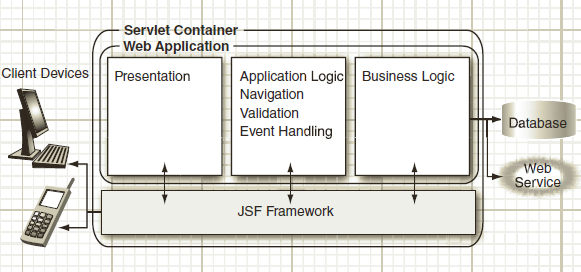
\includegraphics{JSF_architecture.png}
	\caption{Architettura di JSF}
	\label{jsf_arch}
\end{figure}

L'architettura di JSF (illustrata in Figura \ref{jsf_arch} ) segue il classico schema \textit{Model-View-Controller}: JSF consente di collegare il modello (\textit{model}) con l'interfaccia grafica (\textit{view}), fornendo gli strumenti necessari per poter controllare e processare le azioni degli utenti e aggiornare il modello sottostante di conseguenza (\textit{controller}). Tali strumenti realizzano principalmente tre tipi di servizi:

\begin{itemize}
\item \textbf{gestione degli eventi}: interagendo con la pagina web, l'utente può compiere una grande varietà di azioni; esse vengono rilevate dal browser, che \textquoteleft lancia\textquoteright{} il relativo evento. JSF consente di elaborare la risposta del programma tramite un meccanismo molto semplice: è possibile associare ad un dato evento un metodo di un oggetto Java lato server che si occupa della sua gestione.
\item \textbf{conversione dei dati}: nel web, i dati vengono immessi, visualizzati e scambiati sotto forma di stringa; il modello dei dati, invece, è composto da oggetti Java. JSF permette in modo agevole di effettuare le conversioni necessarie per consentire l'interazione tra questi due mondi: oltre a fornire dei convertitori per i tipi basilari (come ad esempio numeri o stringhe), offre anche la possibilità di definire convertitori personalizzati.
\item \textbf{validazione dei dati}: viene realizzata in modo simile alla conversione: lo sviluppatore può decidere di utilizzare i \textit{validator} standard o implementarne di nuovi. Tramite questo meccanismo si evita che gli errori dell'utente pregiudichino la validità del modello.
\end{itemize}


\subsubsection{Bean}

Il livello \textit{controller} di JSF fa un uso intensivo dei \textsl{bean}. Un bean è un oggetto Java gestito dal framework e non in maniera diretta dal programmatore.\\
Esistono vari tipi di bean; quelli a cui si può accedere direttamente da una pagina JSF sono detti \textit{managed bean}. Per essere tale, un bean deve avere un nome ed uno \textit{scope}, ossia un contesto in cui il bean è \textquoteleft visibile\textquoteright{} ed utilizzabile dall'applicazione. \\
Per maggiori dettagli, si rimanda al capitolo INSERIRE RIFERIMENTO A CDI QUI.


\subsection{Funzionamento}

\subsubsection{\textit{Rendering} delle pagine}
Ci sono diversi modi per creare una pagina JSF. Quello standard fa uso della tecnologia \textsl{Facelets}, che è stata sviluppata proprio per essere utilizzata da JSF; per creare una pagina Facelets è infatti sufficiente scrivere un documento XHTML che fa uso dei tag di JSF, con la possibilità di utilizzare l'\textsl{Expression Language} (\textsl{EL}) per consentire la comunicazione tra il livello presentazione e il livello applicazione. Ciascun tag è associato ad una classe che lo gestisce e le istanze di queste classi sono dette \textit{tag handler}: quando la pagina viene letta, i \textit{tag handler} vengono eseguiti e costruiscono un albero dei componenti della pagina (\textit{component tree}). Ad ogni tag corrisponde un nodo dell'albero. Ogni componente è inoltre associato ad un oggetto \textit{renderer}, che produce codice HTML in relazione allo stato del componente stesso (processo che viene detto \textit{encoding}).\\
La pagina così prodotta arriva all'utente. Quando l'utente invia dati al server, questo processa la richiesta e produce una serie di coppie ID/valore che viene memorizzata in una tabella hash. Ciascun componente può quindi consultarla e stabilire quali sono i valori relativi al tag ad esso associato, salvandoli come \textsl{valori locali} (o \textit{local values}). Questa operazione è chiamata \textit{decoding}.\\

\begin{figure}
	\centering
	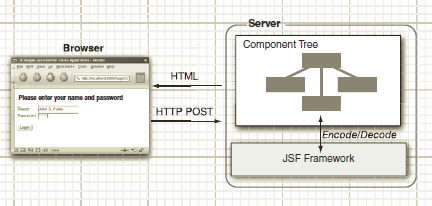
\includegraphics{JSF_client-server_communication.png}
	\caption{\textit{Encoding} e \textit{decoding}}
	\label{jsf_cs_comm}
\end{figure}

\subsubsection{\textit{Comunicazione client-server}}
La comunicazione tra client e server può avvenire essenzialmente in due modi, entrambi standard: tramite richieste \textsl{POST} e \textsl{GET}. JSF inoltre supporta nativamente ed in modo trasparente le richieste AJAX, consentendo di creare pagine web dinamiche. La comunicazione asincrona tramite AJAX è uno strumento molto efficace in vari contesti; la figura \ref{jsf_ajax} mostra come possa ad esempio essere utilizzata per la gestione degli eventi e la validazione dei dati.\\

\begin{figure}
	\centering
	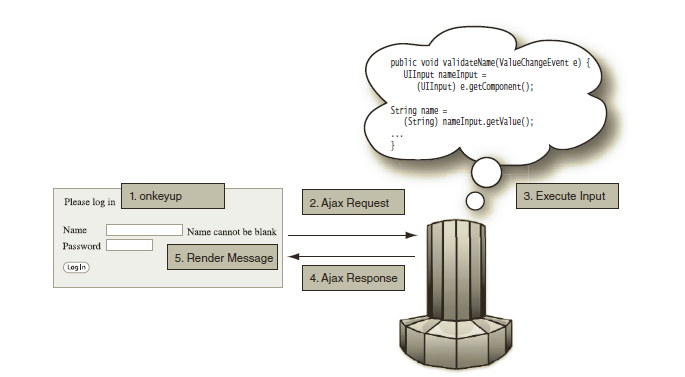
\includegraphics{JSF_ajax.png}
	\caption{Richiesta AJAX per la validazione di un input}
	\label{jsf_ajax}
\end{figure}

\subsubsection{\textit{Ciclo di vita}}
Ciò che viene eseguito tra una richiesta HTTP e la relativa risposta è chiamato dalla specifica JSF \textsl{ciclo di vita} (in inglese \textit{life cycle}).
Di seguito vengono riportate le sei fasi del ciclo di vita di JSF (raffigurate nella figura \ref{jsf_lifecycle}), come stabilito dalla specifica:

\begin{enumerate}
\item \textbf{\textit{Restore view}}: è la fase in cui viene costruito l'albero dei componenti, o viene recuperato nel caso di pagina mostrata precedentemente.
\item \textbf{\textit{Apply request values}}: in questa fase, la richiesta HTTP che l'utente invia al server viene processata, eseguendo l'operazione di \textit{decoding}.
\item \textbf{\textit{Process validations}}: viene eseguita la conversione e la validazione dei dati dell'utente.
\item \textbf{\textit{Update model values}}: durante questa fase viene aggiornato il modello dei dati.
\item \textbf{\textit{Invoke application}}: è la fase in cui il \textit{navigation handler} di JSF decide quale pagina visualizzare in base alle decisioni prese dal controllore.
\item \textbf{\textit{Render response}}: viene eseguito l'\textit{encoding}, producendo una pagina HTML che viene poi inviata al browser tramite la risposta del server.
\end{enumerate}

\begin{figure}
	\centering
	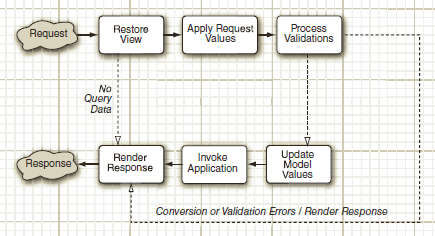
\includegraphics{JSF_life_cycle.png}
	\caption{Ciclo di vita di JSF}
	\label{jsf_lifecycle}
\end{figure}

Non sempre vengono eseguite tutte le fasi del ciclo di vita. Alcuni esempi:

\begin{itemize}
\item Nel caso in cui la richiesta HTTP non contenga valori, a seguito della fase \textit{Restore view} viene eseguita immediatamente la fase \textit{Render response}. Ciò accade, ad esempio, quando una pagina viene visualizzata per la prima volta.
\item Se si riscontrano errori di conversione o validazione durante la fase \textit{Process validations}, si passa alla fase \textit{Render response}: viene visualizzata nuovamente la stessa pagina, mostrando i relativi messaggi di errore (se previsti nella creazione della pagina stessa da parte dello sviluppatore).
\item In una richiesta AJAX vengono indicati quali componenti processare e quali aggiornare. Per i primi vengono eseguite le prime cinque fasi del ciclo di vita e successivamente viene eseguito il \textit{rendering} solo per i componenti da aggiornare.
\end{itemize}

















\section{Deltaspike}
\label{delta}
\textsl{Deltaspike} è un \textit{framework} che estende le funzionalità di \textsl{CDI}. Il suo utilizzo in Jama è la gestione della sicurezza: associare ad ogni utente un insieme di permessi che determinano le azioni che può effettuare.
La caratteristica fondamentale di Deltaspike è l'essere un \textit{framework annotation-based}: funziona tramite le \textsl{Annotation} di Java - che d'ora in poi chiameremo semplicemente annotazioni - il che lo rende facile da utilizzare e poco invasivo.

\subsection{Caratteristiche Generali}
Il cuore della sicurezza in Deltaspike è la classe \textsl{Authorizer}: è un \textit{bean} di CDI - tipicamente \textsl{Application Scoped} - definito dallo sviluppatore che definisce i metodi che verranno invocati durante il controllo sui permessi di un utente. Questi metodi devono essere annotati con l'annotazione \textsl{@Secures} definita da Deltaspike, che indica che essi sono i metodi da invocare per il controllo sui permessi. Non basta: devono essere annotati anche con un'altra annotazione, una \textsl{custom annotation} - cioè definita dallo sviluppatore - che associa il metodo in questione ai metodi su cui effettuare il controllo dei permessi. Quest'ultima deve essere a sua volta annotata con l'annotazione \textsl{@SecurityBindingType} di Deltaspike.\newline
Nonostante già il controllo sui metodi possa essere sufficiente per gestire l'intera sicurezza di un'applicazione, una funzionalità interessante e molto utile di Deltaspike è la possibilità di effettuare un controllo a livello di pagina: ad esempio, far sì che solo un Amministratore possa visitare la pagina di creazione di un utente, o che solo un Operatore Amministrativo possa visitare la pagina di creazione di una convenzione. Inoltre, qualora il controllo non vada a buon fine, si può specificare una pagina di errore diversa per ogni pagina, ed un messaggio di errore che verrà visualizzato a video dopo il redirect.\newline
Per concludere quest'introduzione e visione d'insieme delle funzionalità di Deltaspike con cui abbiamo avuto a che fare, riteniamo comunque importante far notare che, nonostante sia un framework già usabile e utile, non sia ancora completamente maturo: la documentazione è scarsa - per non dire di peggio - e alcune funzionalità utili sono mancanti o non funzionanti - ad esempio, il redirect ad una pagina di errore anche per la sicurezza sui metodi.\newline
Vediamo adesso in dettaglio come utilizzare Deltaspike.



\subsection{Rendere sicuro un metodo}
Per spiegare come si rende sicuro un metodo, prenderemo come esempio un problema che abbiamo affrontato nello sviluppo di Jama: far sì che solo un Operatore Amministrativo possa eliminare una convenzione. L'eliminazione di una convenzione, nella nostra applicazione, consiste in sostanza nell'invocazione di un metodo di uno dei nostri \textit{bean}, quindi il problema si risolve impedendo l'invocazione di tale metodo da parte di utenti che non siano un Operatore Amministrativo.\newline
Il primo passo è il definire un'annotazione, che chiameremo \textsl{@DeleteContractsAllowed}:

\begin{lstlisting}
&&Retention&&(value = RetentionPolicy.RUNTIME)
&&@Target&&({ ElementType.TYPE, ElementType.METHOD })
&&@Documented&&
&&@SecurityBindingType&&
public @interface DeleteContractsAllowed {}
\end{lstlisting}

Procediamo dunque ad annotare il nostro metodo che elimina una convenzione con l'annotazione appena definita:

\begin{lstlisting}
...

&&@DeleteContractsAllowed&&
public void deleteContract() {
	//Elimina una convenzione.
	
	...
}
\end{lstlisting}

L'ultima cosa da fare è fornire l'Authorizer di un metodo annotato \textsl{@Secures} e \textsl{@DeleteContractsAllowed}:

\begin{lstlisting}

public class Authorizer {
	&&@Secures&&
	&&@DeleteContractsAllowed&&
	public boolean canDeleteContracts {
		//Verifica che l'utente possa eliminare una convenzione.
		//Restituisce true in caso affermativo, altrimenti false.
	
		...
	}
}
\end{lstlisting}

Il metodo che abbiamo appena definito verrà invocato da Deltaspike in maniera automatica tutte le volte che si invocherà \textsl{deleteContract()}. Nel caso \textsl{canDeleteContracts()} restituisca \textsl{true}, l'eliminazione può proseguire, altrimenti viene generata un'eccezione.

\subsection{Rendere sicura una pagina} 
La sicurezza su base pagina si implementa definendo interfacce e classi che rappresentano rispettivamente cartelle e pagine. Ad esempio, per rendere sicura la pagina \textsl{home.xhtml} che si trova dentro la cartella \textsl{pages}, definiremo un interaccia \textsl{Pages} con all'interno una classe \textsl{Home}; le classi così definite devono implementare l'interfaccia \textsl{ViewConfig} definita da Deltaspike. Il \textit{path} è relativo alla cartella \textsl{webapp} dell'applicazione, quindi la nostra classe Home contenuta nell'interaccia Pages fa riferimento alla pagina \textsl{webapp/pages/home.xhtml}. I nomi sono \textit{case insensitive}: la classe Home fa riferimento alle pagine home.xhtml e Home.xhtml; stesso discorso vale per le interfacce.\newline
Il metodo più facile per rendere sicuro un insieme di più pagine è creare un file Java e di definire all'interno di quest'ultimo tutta la gerarchia di interfacce e di classi - ricordandoci di omettere il \textit{modifier} \textsl{public} per ognuna delle interfacce/classi, altrimenti si otterrebbe un errore di compilazione.\newline
Ognuna delle classi definite deve essere annotata con l'annotazione \textsl{@Secured}, completata con l'attributo \textsl{value} che specifica una classe definita dallo sviluppatore che implementa l'interfaccia \textsl{AccessDecisionVoter} di Deltaspike; questa classe deve essere un \textit{bean} di CDI, tipicamente \textsl{Application Scoped} .
La classe specificata deve implementare il metodo \textsl{public Set\textless SecurityViolation\textgreater \space checkPermission()}, che viene invocato da Deltaspike ogni volta che si tenta di accedere alla pagina.\newline
Il metodo restituisce un Set di \textsl{SecurityViolation}, una \textsl{Anonymous Inner Class} definita da Deltaspike. Nel caso esso sia vuoto, l'accesso viene consentito, altrimenti viene impedito.\newline Come abbiamo visto nell'introduzione, una delle peculiarità più interessanti della sicurezza su base pagina è il poter specificare una pagina di errore. Per fare ciò, arricchiamo l'annotazione \textsl{@Secured} delle nostre pagine con l'attributo \textsl{errorView}, indicando una pagina definita secondo la solita convenzione spiegata ad inizio paragrafo. Nel caso venga specificata una pagina di errore, le SecurityViolation contenute nel Set restituito da checkPermission() vengono aggiunte al \textit{bundle} di messaggi della pagina, ovvero all'interno dell'area definita dal tag \textsl{\textless h:messages\textgreater} della pagina - detta in maniera meno tecnica, verrà visualizzato un messaggio a video nella pagina di errore per ogni SecurityViolation contenuta. \newline Il messaggio da visualizzare viene specificato nel metodo \textsl{public String getReason()} di ogni SecurityViolation; ricordando che quest'ultima è una Anonymous Inner Class, il metodo getReason() viene obbligatoriamente ridefinito ad ogni SecurityViolation creata, permettendo così di specificare il messaggio di errore più adatto in ogni occasione.\newpage
Per fissare meglio le idee, è opportuno mostrare un esempio. Per prima cosa, creiamo le classi relative alle pagine da rendere sicure:

\begin{lstlisting}
interface Pages {

	@Secured(value = { ViewHomeAccessDecisionVoter.class }, errorView = Login.class)
	class Home implements ViewConfig {}

	
	class Login implements ViewConfig {}

}
\end{lstlisting}

Successivamente definiamo il nostro AccessDecisionVoter; non ci addentreremo nella logica che esegue il controllo, usiamo uno pseudo-codice che renda l'idea di come deve funzionare la classe:

\begin{lstlisting}
&&@ApplicationScoped&&
public class ViewHomeAccessDecisionVoter implements AccessDecisionVoter {
	private SecurityViolation violation = new SecurityViolation() {
		public String getReason() {
			return "Non sei autorizzato";
		};
		
	public Set<SecurityViolation> checkPermission(
				AccessDecisionVoterContext accessDecisionVoterContext) {
				
		Set<SecurityViolation> violations = new HashSet<>();
				
		if( user cannot see home )
			violations.add(violation);
		return violations;
	}
}

\end{lstlisting}
Il gioco è fatto: chiunque tenti di visitare la pagina \textsl{home} senza averne i permessi - ad esempio, un utente che senza fare il login tenta di andare subito alla home - viene reindirizzato alla pagina di login, dove potrà vedere un bel messaggio che recita: \textsl{Non sei autorizzato!}\newline

\section{Altre librerie}
\label{libs}
\subsection{JLDAP}
\label{jldap}
\textsl{LDAP} è un protocollo per l'accesso a cartelle. Definisce un meccanismo in cui i client mandano richieste e ricevono risposte da server LDAP.
\textsl{JLDAP} è una libreria sviluppata da \textsl{Novell} che permette l'accesso al servizio di gestione di cartelle LDAP.

LDAP viene utilizzato dall'applicativo per recuperare, tramite un server LDAP di SIAF, informazioni riguardo agli utenti al momento del login. In particolare consente ai docenti di ateneo di loggarsi con le proprie credenziali uniche di ateneo 
senza che ci sia bisogno di inserirli a mano in qualche database interno.

\paragraph{Funzionamento}
L'operazione centrale è la ricerca dell'utente tramite matricola nel server LDAP. Il metodo che consente di effettuare questa operazione è:

\begin{lstlisting}
 LDAPSearchResults search(String base, int scope, String filter, String[] attrs, boolean typesOnly) 
\end{lstlisting}

I parametri più interessanti di questo metodo sono:
\begin{itemize}
 \item \textsl{base}\\
  Serve per specificare il punto di partenza della query, ovvero la cartella a partire dalla quale effettuare la ricerca. Per l'applicativo tale parametro è impostato a ``ou=people,dc=dinfo,dc=unifi,dc=it'';
  \item \textsl{filter}\\
  Serve per specificare i criteri di ricerca: si specificano i valori di alcuni attributi dell'entità cercata. Nel caso della ricerca per matricola occore impostare ``uid=<matricola>''.
\end{itemize}

Il risultato di questa operazione è una entità rappresentata così:

\begin{lstlisting}
dn: uid=D064678,ou=docenti,ou=personale,ou=people,dc=unifi,dc=it
objectClass: unifiPersonale
cn: NOME COGNOME
gidNumber: 513
uid: D064678
uidNumber: 800064678
employeeType: Professori Associati
givenName: NOME
mail: nome.cognome@unifi.it
sn: COGNOME
userPassword:: {md5}e33ENX1ZdUkzaXNIMSthVEVFejErZUVoM1VRPT1
\end{lstlisting}

Una volta ottenuta l'entità è possibile effettuare il login come spiegato in INSERIRE RIFERIMENTO A LOGIN.

\subsection{FreeMarker}
\label{freemarker}

\textsl{FreeMarker} è un package Java che consente di produrre output testuale basandosi su un template. È stato progettato specificatamente per la generazione automatica di pagine HTML, anche se può creare vari tipi di pagine. La caratteristica principale è che consente di separare la logica che costruisce la pagina con il template in base alla quale viene prodotta; in questo modo, il template è modificabile senza l'intervento di un programmatore (anche se, senza modificare il codice, non è possibile utilizzare informazioni non ricavabili dagli oggetti a cui si ha già accesso).\\
Nei paragrafi che seguono verrà descritto il package FreeMarker e spiegato come è stato usato all'interno dell'applicazione. Per maggiori informazioni su questo tool, si rimanda alla pagina web relativa al progetto \cite{freemarker}, dalla quale sono stati presi - fra l'altro - gli esempi sul funzionamento e utilizzo del software.


\subsubsection{Funzionamento}
Per il funzionamento di FreeMarker sono necessari due elementi:
\begin{itemize}
\item un file di template
\item i parametri con cui \textquotedblleft riempire\textquotedblright{} il template, che costituiscono il \textit{data model}.
\end{itemize}

\paragraph{\textit{Data model}}
Come parametri possono essere usate varie classi Java:

\begin{itemize}
\item \lstinline{String} per le stringhe
\item \lstinline{Number} per i numeri
\item \lstinline{Boolean} per i booleani
\item \lstinline{List} o gli array Java per sequenze di valori
\item \lstinline{Map} o bean per coppie chiave-valore (dette \textsl{hash}, come si vedrà fra poco)
\end{itemize}

Passati questi parametri, FreeMarker costruisce il \textit{data model}, che è essenzialmente un albero così formato:

\begin{itemize}
\item la radice è un nodo speciale chiamato, appunto, \textit{root}
\item i nodi intermedi, chiamati anche \textsl{variabili}, possono essere:
\begin{itemize}
\item \textit{hashes} se i loro figli sono identificati tramite nomi
\item \textit{sequences} se i figli sono identificati tramite un indice sequenziale che inizia da 0 (i.e., sono l'equivalente di un array)
\end{itemize}
In entrambi i casi, i loro figli vengono detti \textit{subvariables}
\item le foglie sono dette \textit{scalars}.
\end{itemize}

Ad esempio:

\begin{lstlisting}
(root)
  |
  +- animals
  |   |
  |   +- mouse
  |   |   |   
  |   |   +- size = "small"
  |   |   |   
  |   |   +- price = 50
  |   |
  |   +- elephant
  |   |   |   
  |   |   +- size = "large"
  |   |   |   
  |   |   +- price = 5000
  |   |
  |   +- python
  |       |   
  |       +- size = "medium"
  |       |   
  |       +- price = 4999
  |
  +- test = "It is a test"
  |
  +- whatnot
        |
        +- fruits
            |
            +- (1st) = "orange"
            |
            +- (2nd) = "banana"
\end{lstlisting}

In questo \textit{data model}:

\begin{itemize}
\item \lstinline{animals}, \lstinline{mouse}, \lstinline{elephant}, \lstinline{python} e \lstinline{whatnot} sono \textit{hashes}
\item \lstinline{fruits} è una \textit{sequence}
\item tutti gli altri nodi eccetto \textit{root} sono foglie
\item \lstinline{mouse} ha come \textit{subvariables} \lstinline{size} e \lstinline{price} (così come anche \lstinline{elephant}, ad esempio).
\end{itemize}


\paragraph{Template} 
Un file di template è un semplice file di testo (di qualunque tipo) in cui sono presenti delle variabili. Per inserire una variabile, la sintassi è:

\begin{lstlisting}
${nome}
\end{lstlisting}

Un esempio di file di template (nello specifico, si tratta di un file HTML) è il seguente:

\begin{lstlisting}
<html>
<head>
  <title>Welcome!</title>
</head>
<body>
  <h1>Welcome ${user}!</h1>
  <p>Our latest product:
  <a href="${latestProduct.url}">${latestProduct.name}</a>!
</body>
</html>
\end{lstlisting}

\paragraph{Output}
Una volta che si ha un file di template e un \textit{data model} opportuno, si cercano all'interno del modello nodi con lo stesso nome delle variabili inserite nel programma e si sostituisce il valore della variabile nel template con quello della variabile nel modello (questa sostituzione viene detta \textsl{interpolazione}). Se nel template si fa riferimento ad una proprietà di una variabile, si cerca quella proprietà fra le \textit{subvariables} della variabile nel modello. Ad esempio, considerando il template precedente ed un \textit{data model} così composto:

\begin{lstlisting}
(root)
  |
  +- user = "Big Joe"
  |
  +- latestProduct
      |
      +- url = "products/greenmouse.html"
      |
      +- name = "green mouse"  
\end{lstlisting}

l'output sarà il file:

\begin{lstlisting}
<html>
<head>
  <title>Welcome!</title>
</head>
<body>
  <h1>Welcome Big Joe!</h1>
  <p>Our latest product:
  <a href="products/greenmouse.html">green mouse</a>!
</body>
</html>
\end{lstlisting}

\subsubsection{Utilizzo}
Per utilizzare FreeMarker bisogna innanzitutto creare una configurazione tramite la classe \lstinline{Configuration}, specificando, tra le altre cose, la directory in cui si trovano i template e la codifica da adoperare.\\
In seguito, bisogna definire il modello. Per fare ciò è possibile usare diverse classi Java, a seconda del tipo di variabile da inserire; tipicamente, si utilizzano mappe o bean.\\
Infine, si crea un oggetto di tipo \lstinline{Template}, lo si inizializza con il template desiderato e si produce l'output tramite la chiamata al metodo \lstinline{process} dell'oggetto \lstinline{Template}, la cui signature è:

\begin{lstlisting}
public void process(java.lang.Object dataModel, java.io.Writer out) throws TemplateException, java.io.IOException
\end{lstlisting}

dove \lstinline{dataModel} è ovviamente il modello e \lstinline{out} è il \lstinline{Writer} sul quale produrre il risultato.\\
Di seguito è riportato un esempio di un'applicazione che esegue il processo appena descritto:

\begin{lstlisting}
import freemarker.template.*;
import java.util.*;
import java.io.*;

public class Test {

    public static void main(String[] args) throws Exception {
        
        /* ----------------------------------------------------------------------- */    
        /* You should do this ONLY ONCE in the whole application life-cycle:       */    
    
        /* Create and adjust the configuration */
        Configuration cfg = new Configuration();

        cfg.setDirectoryForTemplateLoading(new File("/where/you/store/templates"));
        cfg.setObjectWrapper(new DefaultObjectWrapper());
        cfg.setDefaultEncoding("UTF-8");
        cfg.setTemplateExceptionHandler(TemplateExceptionHandler.HTML_DEBUG_HANDLER);
        cfg.setIncompatibleImprovements(new Version(2, 3, 20));

        /* ----------------------------------------------------------------------- */    
        /* You usually do these for many times in the application life-cycle:      */    

        /* Create a data-model */
        Map root = new HashMap();
        root.put("user", "Big Joe");
        Map latest = new HashMap();
        root.put("latestProduct", latest);
        latest.put("url", "products/greenmouse.html");
        latest.put("name", "green mouse");

        /* Get the template */
        Template temp = cfg.getTemplate("test.ftl");

        /* Merge data-model with template */
        Writer out = new OutputStreamWriter(System.out);
        temp.process(root, out);
    }
}
\end{lstlisting}


\chapter{Test funzionale e collaudo}
Questo capitolo è una sorta di manuale dell'utente: illustra come utilizzare ognuna delle funzionalità dell'applicazione. In Figura \ref{jama_home} è raffigurata la pagina principale di Jama, da cui si possono effettuare tutte le azioni disponibili in base all'utente loggato. La figura illustra la pagina principale per un Operatore; un Docente, per esempio, vedrebbe solo il tasto ''Visualizza i contratti''.
\begin{figure}[h]
	\centering
	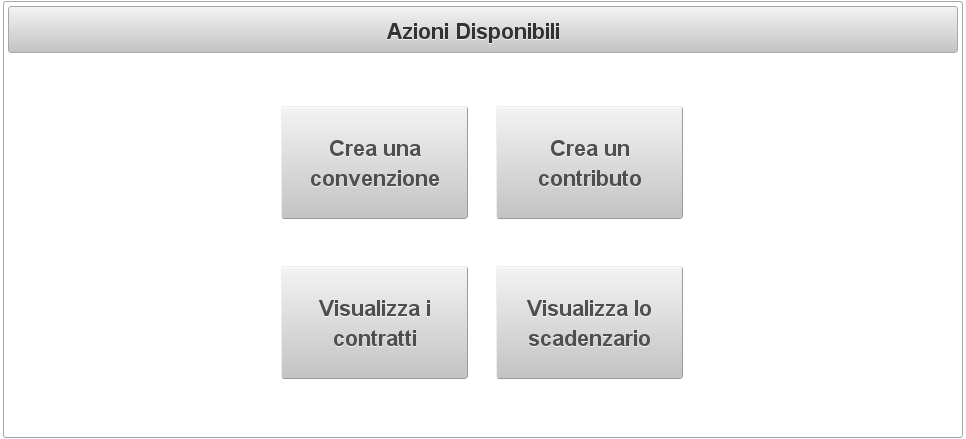
\includegraphics[width=13cm,height=6.5cm]{jama_home.png}
	\caption{La pagina principale di Jama}
	\label{jama_home}
\end{figure}

\section{Creare una convenzione}
\paragraph{}
Per creare una convenzione si clicca sul tasto ''Crea una convenzione''. Apparirà la finestra di Figura \ref{jama_create_agreement_tab_data}, in cui l'Operatore può inserire i dati principali della convenzione. Cliccando sul pulsante ''Next'', apparirà la finestra di Figura \ref{jama_create_agreement_tab_sharetable}, in cui l'utente può inserire i dati della Tabella di Ripartizione. Cliccando sul pulsante ''Annulla'', come si può intuire, l'inserimento della convenzione viene annullato e si ritorna alla pagina principale.\newline
Tornando alla Figura \ref{jama_create_agreement_tab_data}, accanto al menù ''Responsabile Scientifico'' è presente il pulsante ''Aggiungi'' che, se cliccato, farà apparire il pop-up di Figura \ref{jama_chief_scientist_popup}, che consente di inserire un nuovo Responsabile Scientifico all'interno dell'applicazione. Il campo ''Matricola'' del pop-up serve ad associare tale Responsabile Scientifico all'utente che effettivamente è legato ad esso; ad esempio, se la matricola del Professor Enrico Vicario è D593, inserendo il Responsabile Scientifico ''Enrico Vicario'' con matricola ''D593'' il Professor Vicario, effettuando il login con la sua matricola, potrà consultare le sue effettive convenzioni.\newline
Il pulsante ''Aggiungi'' accanto al menù delle Ditte è simile al precedente, con l'unica differenza che le Ditte non hanno matricola e non sono associate ad alcun utente.\newline

\begin{figure}[h]
	\centering
	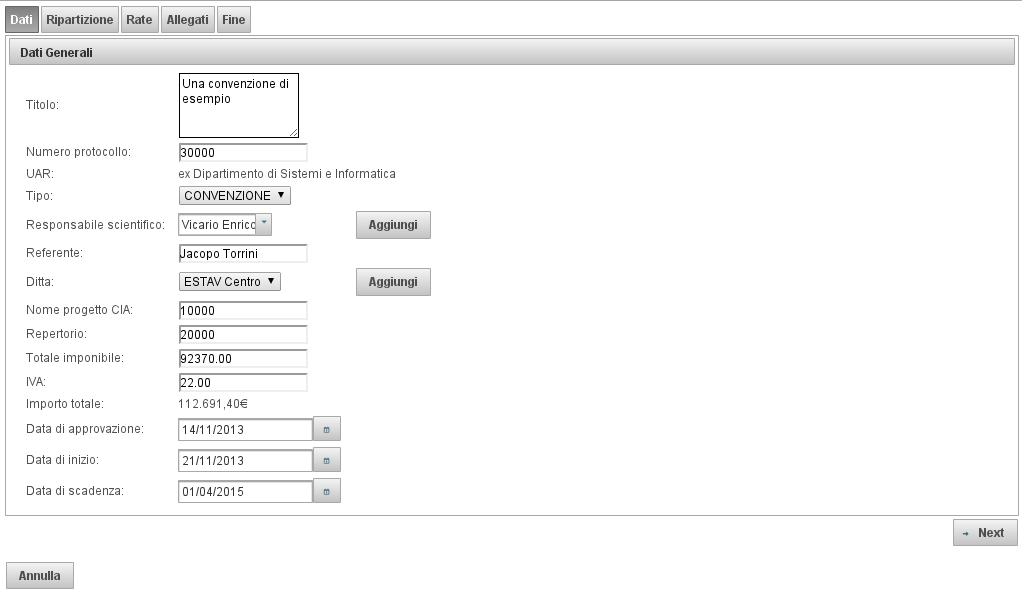
\includegraphics[width=13cm,height=6.5cm]{jama_create_agreement_tab_data.png}
	\caption{I dati principali di una convenzione}
	\label{jama_create_agreement_tab_data}
\end{figure}

\paragraph{}
Tornando alla Tabella di Ripartizione - Figura \ref{jama_create_agreement_tab_sharetable} - qualora la quota del ''Personale'' sia diversa da 0, si dovrà specificare almeno un Responsabile Scientifico nella tabella in fondo alla pagina. Per fare ciò, si seleziona il Responsabile Scientifico e la sua quota, e si clicca sul pulsante ''Aggiungi''. Com'è ovvio, sommando le quote della tabella si deve ottenere il 100\%, altrimenti verrà segnalato un errore e non si potrà continuare l'inserimento.\newline
Nel caso in cui si voglia cambiare un Responsabile Scientifico o la sua quota, si dovrà prima rimuovere la riga della tabella tramite il pulsante ''Rimuovi'', per poi inserire la nuova quota.\newline
Cliccando il pulsante ''Next'' si arriverà alla schermata della gestione delle rate, illustrata in Figura \ref{jama_installment_management}.
\paragraph{}
\begin{figure}
	\centering
	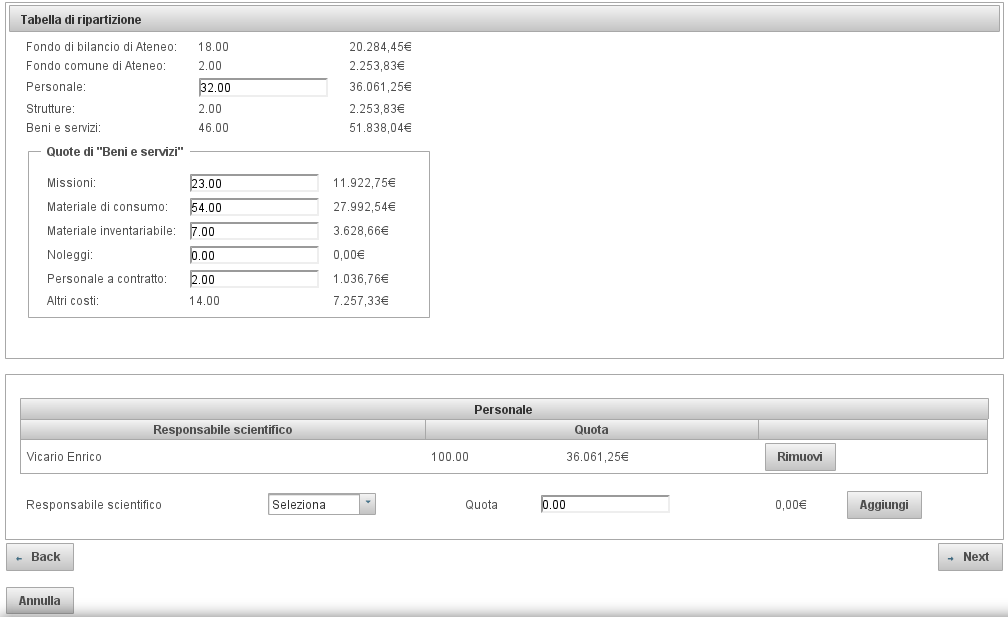
\includegraphics[width=13cm,height=6.5cm]{jama_create_agreement_tab_sharetable.png}
	\caption{La tabella di ripartizione}
	\label{jama_create_agreement_tab_sharetable}
\end{figure}

\begin{figure}
	\centering
	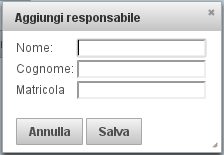
\includegraphics{jama_chief_scientist_popup.png}
	\caption{Il pop-up per inserire un nuovo Responsabile Scientifico nel database}
	\label{jama_chief_scientist_popup}
\end{figure}
La pagina di gestione delle rate è molto semplice: in alto vi è la lista delle rate della convenzione, che si inseriscono, prevedibilmente, con il pulsante ''Aggiungi una rata''. Parleremo in dettaglio di come si aggiunge una rata nei paragrafi successivi.\newline
Cliccando il pulsante ''Next'', si arriva alla pagina degli allegati, mostrata in Figura \ref{jama_attachments_management}.
\paragraph{}
La schermata di gestione degli allegati è fondamentalmente identica a quella delle rate: in alto è presente la lista a cui aggiungere gli allegati tramite il pulsante ''Aggiungi''.\newline
Gli allegati inseriti si possono cancellare e scaricare rispettivamente attraverso i due bottoni visibili in figura, che appaiono
andando col mouse sopra la riga in questione.
\paragraph{}
Infine, cliccando ancora una volta sul pulsante ''Next'' - sì, si fa presto a diventare ripetitivi a scrivere un manuale utente - si arriva alla schermata conclusiva, mostrata in Figura \ref{jama_agreement_save}. Cliccando sul pulsante ''Salva'', la convenzione viene finalmente registrata.

\begin{figure}
	\centering
	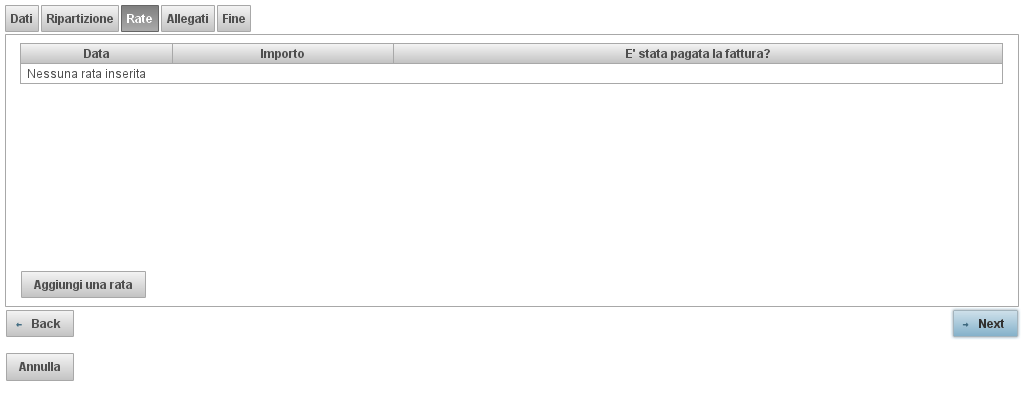
\includegraphics[width=13cm,height=6.5cm]{jama_installment_management.png}
	\caption{La pagina di gestione delle rate}
	\label{jama_installment_management}
\end{figure}

\begin{figure}
	\centering
	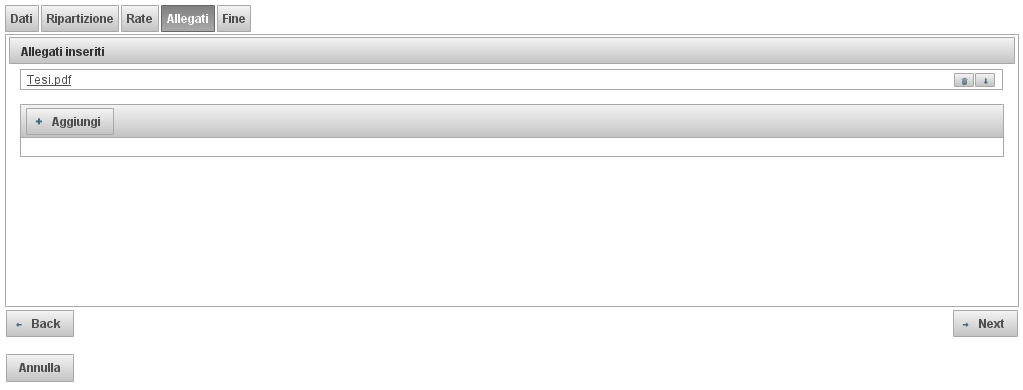
\includegraphics[width=13cm,height=6.5cm]{jama_attachments_management.png}
	\caption{La pagina di gestione degli allegati}
	\label{jama_attachments_management}
\end{figure}

\begin{figure}
	\centering
	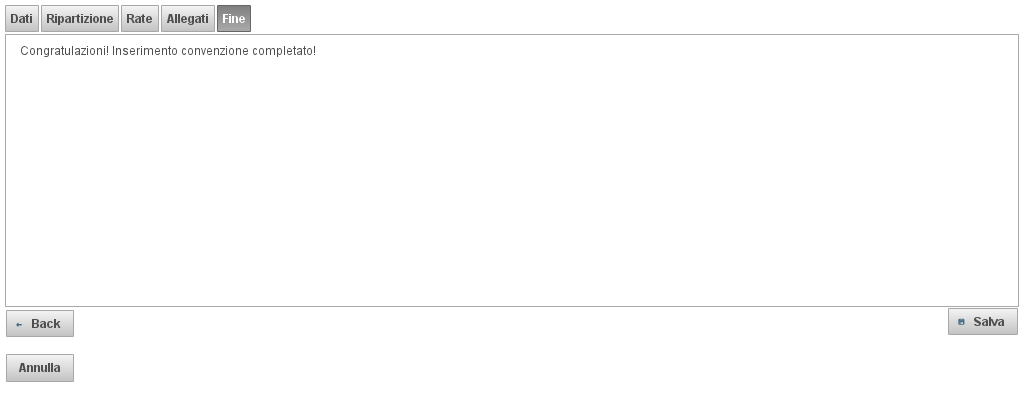
\includegraphics[width=13cm,height=6.5cm]{jama_agreement_save.png}
	\caption{La pagina conclusiva}
	\label{jama_agreement_save}
\end{figure}


\label{howto}
\chapter{Dietro le quinte}
\label{code}
\section{Login}
\label{login}


La schermata di login si presenta in maniera molto semplice: è costituita da un messaggio di benvenuto e da un form in cui inserire le proprie credenziali per poter accedere. I dati inviati dal form vengono processati dal bean \lstinline{UserManager}, che si occupa di eseguire l'autenticazione.\\
Quando l'utente invia il form viene chiamato il metodo \lstinline{login} dello \lstinline{UserManager}, listato qui di seguito:

\begin{lstlisting}
public String login(String password) {
		User u = userDao.getBySerialNumber(insertedSerialNumber);
		try {
			if (!(u == null || !u.login(password))) {
				loggedUser = new Principal(u);
				System.out.println("User Login: loggedUser= " + u);
				return "home";
			} else {
				FacesMessage msg = Messages.getMessage("info_badLogin");
				msg.setSeverity(FacesMessage.SEVERITY_INFO);
				FacesContext.getCurrentInstance().addMessage(null, msg);
				
				return "login";
			}
		} catch (IllegalStateException e) {
			return "error";
		}
	}
\end{lstlisting}

Per prima cosa, il sistema recupera l'utente associato alla matricola inserita tramite il DAO \lstinline{UserDaoBean}. Esso esegue un'interrogazione al database locale; se non trova nessuna corrispondenza, il compito di cercare la matricola viene delegato  allo \lstinline{LdapManager}, il quale effettua una ricerca nel sistema di autenticazione di Ateneo utilizzando il protocollo LDAP per la comunicazione. Se anche in questo caso non viene trovato un riscontro, l'utente viene avvertito con un messaggio di errore.\\
Se invece viene trovato un utente, tutte le informazioni ad esso relative vengono salvate in un oggetto \lstinline{User} che viene restituito allo \lstinline{UserManager}. A questo punto viene verificata la validità della password. Questo compito è delegato alla classe \lstinline{User} stessa, la quale contiene al suo interno un attributo di tipo \lstinline{Encryptor} che specifica l'algoritmo di criptazione utilizzato per la propria password. La password inserita viene quindi criptata e confrontata con quella memorizzata. Chiaramente, si procede solo se risultano uguali.\\
A questo punto lo \lstinline{UserManager} crea un nuovo \lstinline{Principal} con i dati dell'utente e viene mostrata la home dell'applicazione: il login è stato effettuato con successo!
\section{Recupero degli Utenti}
La classe che si occupa del recupero degli utenti è \texttt{UserDaoBean}: è possibile recuperare gli utenti sia dal database interno sia sfruttando il servizio LDAP in modo del tutto trasparente.
Il database ha priorità rispetto ad LDAP in modo che sia possibile sovrascrivere alcune informazioni sugli utenti semplicemente inserendoli nel database. Per quanto riguarda il recupero dal database è sufficiente una query per matricola 
mentre per ottenere i dati dal server LDAP è necessario effettuare qualche operazione in più, perciò il codice che compie questa operazione è stato incapsulato in una classe chiamata \texttt{LdapManager}.

Tale classe effettua la connessione al server LDAP tramite il protocollo sicuro \textsl{ldaps} e successivamente sfrutta il metodo \texttt{search(...)} come visto in INSERIRE RIFERIMENTO per ottenere i dati sull'utente in base alla sua matricola.
Tale ricerca è effettuata impostando il parametro \textsl{base} a ``ou=people, dc=dinfo, dc=unifi, dc=it''e \textsl{filter} a ``uid= <matricola> ''. Il parametro base viene letto dal file di configurazione 
\path{standalone/deployments/Jama.war/WEB-INF/classes/config/ldap.properties}, quindi è possibile cambiarlo in qualsiasi momento se lo schema esposto dal server LDAP dovesse cambiare.
A partire dai dati contenuti nel \texttt{LDAPSearchResults} restituito da \texttt{search(...)} è possibile istanziare la classe \texttt{User} che rappresenta un utente.

Il metodo di \texttt{UserDaoBean} che restituisce un utente in base alla matricola è riportato qui sotto.

\begin{lstlisting}
public User getBySerialNumber(String serialNumber) {
	User result = null;
	
	try {
		result = em.createNamedQuery("User.findBySerialNumber", User.class).setParameter("number", serialNumber).getSingleResult();
		
		if (null == result) {
			result = ldapm.getUser(serialNumber);
		}
		
	} catch (NoResultException e) {
		result = null;
	}

	return result;

}
\end{lstlisting}




\section{Lista convenzioni}
\subsection{Livello presentazione}

All'interno dell'applicazione, ricoprono un ruolo centrale le schermate di visualizzazione delle convenzioni/contributi. Gli oggetti che consentono il funzionamento di una schermata di visualizzazione della convenzione sono i seguenti:

\begin{itemize}
\item il file \texttt{.xhtml} che produce la pagina web
\item un bean \textsl{controllore di pagina}
\item un \textit{lazy model}, che rappresenta i dati visualizzati
\item un DAO che recupera i dati da visualizzare
\end{itemize}

Di seguito, segue una spiegazione di ognuno di questi componenti.

\subsubsection{Pagina web}
Una schermata di visualizzazione delle convenzioni/contributi è costituita essenzialmente da una tabella, che viene creata mediante il tag \lstinline{pdata:Table} di PrimeFaces. Poiché dovrà gestire grandi quantità di dati, è stata utilizzata la paginazione unita al \textit{lazy loading}: quando viene caricata una pagina, vengono mantenuti in memoria soltanto i contratti che vengono effettivamente visualizzati. Ciò è reso possibile (o, perlomeno, molto più semplice) grazie ai due attributi della \texttt{dataTable} di PrimeFaces \texttt{paginator} e - soprattutto - \texttt{lazy}; sono entrambi attributi booleani che specificano se utilizzare la relativa tecnica.

\subsubsection{Controllore di pagina}
Associata ad ogni vista, vi è un bean detto \textsl{controllore di pagina}. Esso si occupa di gestire la conversazione necessaria al corretto funzionamento della pagina e di fare da intermediario tra la vista ed il modello, eseguendo le operazioni necessarie per eseguire la navigazione verso le varie schermate dell'applicazione raggiungibili. Il controllore di pagina ha due attributi importanti: il \textit{lazy model}, a cui si può far riferimento dalla pagina, e un \lstinline{ContractManager} che invece si occupa della logica di business, gestendo i contratti (e che non è direttamente accessibile dalla pagina).

\subsubsection{\textit{Lazy model}}
Per creare una tabella \textit{lazy-loaded}, è necessario implementare un \textit{lazy model}, che fornirà la lista di oggetti che verranno infine visualizzati. Il \textit{lazy model} deve inoltre gestire gli eventuali filtri ed ordinamenti richiesti.\\
Un \textit{lazy model} è una classe Java che estende la classe di PrimeFaces \lstinline{LazyModel<T>}, dove \texttt{T} è il tipo di dati da visualizzare (in questo caso, quindi, bisognerà estendere \lstinline{LazyModel<Contract>}). Il metodo principale di questa classe è \lstinline{load}, che ha il compito di caricare i dati dal modello e passarli alla tabella. La sua signature è:

\begin{lstlisting}
public List<T> load(int first, int pageSize, String sortField, SortOrder sortOrder, Map<String, String> filters)
\end{lstlisting}

Questo metodo viene chiamato ogni volta che bisogna aggiornare la tabella. I parametri formali rappresentano:

\begin{enumerate}
\item \texttt{first} e \texttt{pageSize}: la prima riga da visualizzare (partendo da 0) e la dimensione di una pagina, rispettivamente. Queste due informazioni possono essere combinate per sapere quale pagina è visualizzata correntemente: è infatti il quoziente della divisione intera di \texttt{first} per \texttt{pageSize}.
\item \texttt{sortField, sortOrder}: sono informazioni sull'ordinamento della tabella. Il primo indica in base a quale campo ordinare, il secondo è un'enumerazione che indica se l'ordinamento deve essere ascendente o discendente.
\item \texttt{filters}: è una mappa di coppie in cui la chiave è il campo su cui filtrare e il valore è, appunto, il valore del campo.
\end{enumerate}

Affinché la paginazione sia effettivamente \textit{lazy}, però, è necessario che la query effettuata per ottenere le informazioni sia \textquoteleft mirata\textquoteright{}. Per maggiori dettagli su come questo avvenga, si rimanda alla sezione \ref{list_business}.

Se la tabella prevede anche che una riga possa essere selezionata, un \textit{lazy model} deve anche esporre i metodi \lstinline{getRowData} e \lstinline{getRowKey}, che consentono, rispettivamente, di estrarre il dato relativo ad una riga e la riga relativa ad un dato. Entrambi utilizzano una chiave fornita dal programmatore per distinguere le righe della tabella (come ad esempio un identificativo) che deve essere esplicitata nell'attributo \texttt{rowKey} della \lstinline{p:dataTable}.

\paragraph{\textit{Lazy model} delle liste di contratti}
Molte liste di contratti, da quelle visualizzate dall'Operatore a quella a cui ha accesso il Docente, condividono varie operazioni in comune e sono state perciò create classi astratte per il riuso del codice.\\
La classe di base è \lstinline{ContractTableLazyDataModel}, che è un \textit{lazy model} e implementa tutte le operazioni precedentemente descritte, consentendo perciò il normale funzionamento dell'interfaccia. Tuttavia, tramite una lista di contratti è possibile svolgere alcune operazioni che comportano la navigazione ad un'altra pagina web (un esempio è la visualizzazione della convenzione). Quando l'utente ritorna alla lista, la pagina viene creata \textit{ex-novo} e la tabella non mantiene perciò i cambiamenti effettuati dall'utente, come ad esempio il filtraggio dei risultati in base alla data. \\
La classe \lstinline{ContractTableLazyDataModel} risolve questi problemi, esponendo dei metodi per impostare o estrarre lo stato della tabella. L'intero procedimento avviene in questo modo:

\begin{enumerate}
\item l'utente esegue un'operazione su una convenzione che comporta il cambio di pagina, come la visualizzazione o la modifica
\item viene chiamato il rispettivo metodo del controllore di pagina, che estrae lo stato della tabella come una stringa di coppie chiave/valore e lo passa al bean del livello sottostante che si occupa della gestione dei contratti (il \lstinline{ContractManager})
\item la conversazione attuale viene chiusa
\item il \lstinline{ContractManager} inizia una nuova conversazione
\item la nuova pagina viene visualizzata; a questo punto il controllore di pagina precedente è \textit{out of scope}
\item l'utente esegue alcune operazioni nella nuova pagina e poi clicca sul pulsante per tornare alla lista, causando la chiusura della conversazione
\item all'URL prodotto per tornare alla tabella vengono accodati i parametri passati precedentemente al \lstinline{ContractManager} come stringa
\item prima che la pagina sia caricata, il bean controllore di pagina viene inizializzato dal container: la conversazione comincia e il \textit{lazy model} viene creato
\item il \textit{lazy model} viene inizializzato con i parametri contenuti nell'URL
\item la pagina viene caricata e la tabella ritorna così allo stato in cui si trovava prima della visualizzazione/modifica.
\end{enumerate}
\paragraph{Pager e Criteria API}

La classe che si occupa del recupero delle informazioni dal database è \texttt{ContractSearchService}. Lo scopo di questa classe è effettuare un ricerca paginata sul database secondo vari criteri di ricerca quali 
responsabile scientifico, data, dittà etc. Il codice che si occupa della paginazione è stato incapsulato nella classe \texttt{ResultPager}. \texttt{ResultPager} viene costruito
col metodo

\lstinline{ResultPagerBean(int currentPage, int pageSize, TypedQuery<T> query, TypedQuery<Long> countQuery)}

Come si può vedere è possibile impostare il numero di risultati per ogni pagina, la pagina corrente e naturalmente la query che si vuole eseguire. Per ottenere una pagina di risultati è sufficiente chiamare \lstinline{getCurrentResults()}
mentre è possibile spostarsi da una pagina all'altra tramite \lstinline{next()} e \lstinline{previous()}

\texttt{ContractSearchService} viene specializzato, per poter eseguire la paginazione, tramite la composizione con un oggetto di tipo \texttt{Pager}, l'interfaccia che \texttt{ContractSearchService} e \texttt{ResultPager} implementano, come
illustrato in figura \ref{pager}


\begin{figure}[h]
  \caption{Digramma delle classi per Pager}
  \label{pager}
  \centering
    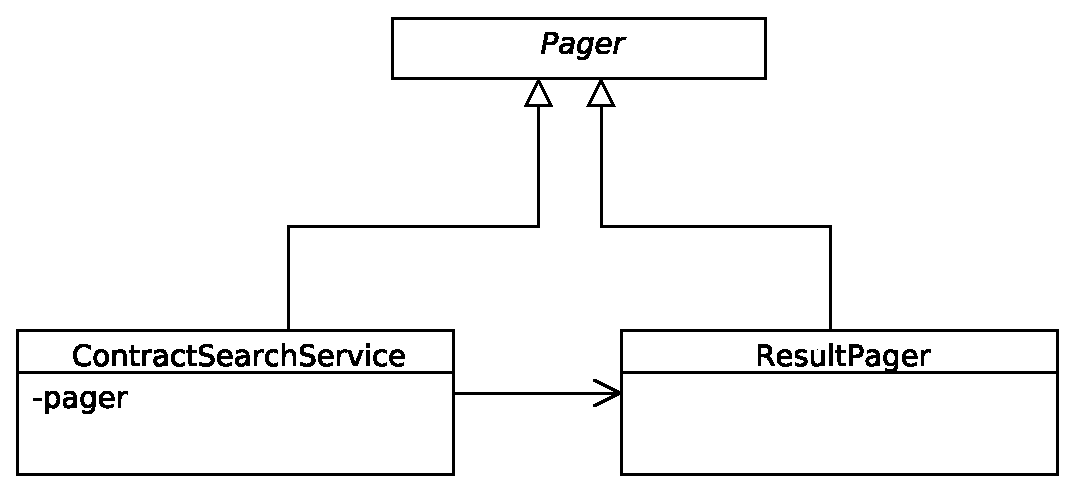
\includegraphics[width=0.7\textwidth]{pager.eps}
\end{figure}

La query è invece costruita utilizzando le Criteria API di JPA, un modo alternativo per costruire query che usa una API java invece di un linguaggio
come JPQL. Questo tipo di costruzione è specialmente indicata per query dinamiche, ovvero quando non si conoscono i criteri di ricerca fino al runtime.
Il caso che si sta analizzando è proprio quello di una query dinamica: l'utente tramite l'interfaccia messa a disposizione filtra le convenzioni/contributi
in base a vari tipi di criteri.

Volendo usare JPQL si sarebbe dovuto costruire la stringa di definizione della query al runtime, passarla al metodo \lstinline{createQuery} di un
\texttt{Entity Manager} il quale avrebbe parsato la stringa e restituito un oggetto \texttt{Query} da cui sarebbe stato possibile estrarre i risultati.
Ciò significa che ogni volta che si vuole eseguire query è necessario parsare una stringa, costruendo una rappresentazione interna della query per poi generare il codice SQL da
eseguire sul database. Criteria API consente di eliminare l'overhead dovuto al parsing e costruire i vari criteri di ricerca utilizzando una API Java invece
di stringhe. Di seguito è mostrato un estratto di codice usato in \texttt{ContractSearchService} per definire la query.

\begin{lstlisting}

TypedQuery<Contract> query;

CriteriaBuilder cb = em.getCriteriaBuilder();
CriteriaQuery<Contract> c = cb.createQuery(Contract.class);
Root<? extends Contract> agr = c.from(contractClass);

c.select(agr).distinct(true);

List<Predicate> criteria = new ArrayList<Predicate>();

if (companyId != null) {

	ParameterExpression<Integer> p = cb.parameter(Integer.class,
			"companyId");
	criteria.add(cb.equal(agr.get("company").get("id"), p));

}

...


c.where(cb.and(criteria.toArray(new Predicate[0])));
	
query = em.createQuery(c);

if (companyId != null) {
	query.setParameter("companyId", companyId);
	countQuery.setParameter("companyId", companyId);

}

...	

 
\end{lstlisting}

Come si può vedere dall'estratto, per prima cosa si crea una query Root, questa gioca il ruolo di una variabile identificativa in una clausola FROM 
in JPQL e indica a quale tipo di schema si è interessati; quindi con l'operazione \lstinline{select(agr)} si indica quale è il
risultato della query. La clausola WHERE è invece ottenuta componendo una serie di predicati, per esempio con l'espressione
\lstinline{cb.equal(agr.get("company").get("id"), p)} si richiede che l'id della dittà sia uguale ad un certo valore.




\section{Creazione e Modifica di Entità}

Il processo di creazione di un entità del modello coinvolge vari componenti:

\begin{itemize}
\item una pagina web che viene utilizzata nella creazione dell'interfaccia grafica
\item (opzionale) un bean di presentazione, che garantisce un corretto funzionamento della pagina
\item un controllore, che fa da intermediario tra il livello di presentazione e il modello di business
\item un DAO, che si occupa della comunicazione con il database
\end{itemize}

\subsection{Livello presentazione}

Quando una schermata di creazione viene visualizzata, per prima cosa viene istanziato dal \textit{container} il controllore che si occupa della creazione dell'entità, il quale a sua volta inizia una conversazione e crea l'oggetto che conterrà i valori immessi tramite interfaccia dall'utente.\\
Graficamente, le pagine web di questo tipo sono costituite semplicemente da alcuni campi di input, inseriti all'interno di un wizard se il numero di valori da inserire è troppo elevato e renderebbe troppo carica un'unica schermata; in questo caso, si rende a volte necessario un bean di presentazione per controllare il flusso del wizard. Normalmente, i form non sono inseriti direttamente nella pagina; piuttosto, si utilizzano vari componenti personalizzati, i quali vengono inclusi nella pagina per ottenere l'effetto desiderato. In questo modo, lo stesso componente può essere utilizzato in più contesti. Questo è reso possibile grazie al tag \lstinline{composite} di JSF, che consente di creare componenti ed inserirle all'interno di un namespace personalizzato.\\
La pagina è poi ovviamente corredata di pulsanti per salvare i dati inseriti o per tornare alla vista precedente ignorando i cambiamento. Nel caso in cui l'utente decida di salvare le modifiche effettuate, il controllore provvede ad aggiornare il database per mezzo del DAO opportuno. In entrambi i casi, la conversazione viene chiusa e si ritorna alla schermata precedente.
\subsection{Edit Session e Extended Persistence Context}
Si descrive la struttura di un bean, da qui in avanti \texttt{Manager}, che possa essere usato dallo strato di presentazione per la creazione e modifica di una entità di business.

\paragraph{Caratteristiche del Manager}
\texttt{Manager} avrà un riferimento all'entità di business che stiamo creando o modificando che possa essere riempita in base ai campi riempiti dall'utente a video.
Come si è detto la creazione/modifica di una entità di business in generale è realizzata attraverso più passi di una procedura, e quindi non può essere confinata in una sola request. Questo suggerisce che \texttt{Manager} debba essere 
\textsl{request scoped}. Si sottolinea che non sarebbe possibile usare un bean di tipo \textsl{session scoped} perché questo comporterebbe la condivisione del bean fra due tab del browser: l'utente che crede di creare due entità in parallelo
sta invece modificando la stessa!

Direttamente collegato alla questione dello scope c'è il problema del detachment: se il Persistence Context che viene usato ha il proprio ciclo di vita legato alla transazione, necessariamente dopo il recupero dal database l'entità diventerà
detached. Questo problema si pone in realtà solo nel caso della modifica, per la creazione infatti possiamo pensare di persistere l'entità solo al termine della procedura. Come si è spiegato in \ref{jpa} lo stato di un entità detached non verrà scritto sul database in nessuna transazione. Sebbene sia possibile riportare un' entità da detached a managed tramite
l'operazione di \texttt{merge()}, in generale è preferibile non farlo perché la gestione dei riferimenti dell'entità è problematica. Per ovviare a questo problema possiamo optare per un Entity Manager di tipo extended. Questo ci garantisce
che durante tutto il ciclo di vita del bean \texttt{Manager}, ovvero per tutta la conversation, avremmo un solo Persistence Context, e di conseguenza l'entità che stiamo modificando non sarà mai detached.

Un'altra problematica che si deve affrontare è prevedere la possibilità di annullare la creazione/modifica in qualsiasi momento della procedura. Per risolvere questo problema dobbiamo gestire le transazioni del container.
Un modo elegante per farlo è annotare il bean con l'annotazione 
\begin{lstlisting} 
@TransactionAttribute(TransactionAttributeType.NOT_SUPPORTED)
\end{lstlisting}
e il metodo che conclude la procedura salvando i dati con 
\begin{lstlisting}
@TransactionAttribute(TransactionAttributeType.REQUIRES_NEW)
\end{lstlisting}



Il bean \texttt{Manager} può quindi essere strutturato come segue:

\begin{lstlisting}
 
@ConversationScoped
@Stateful
@TransactionAttribute(TransactionAttributeType.NOT_SUPPORTED)
public class Manager implements Serializable {

	private static final long serialVersionUID = -4966124878956728047L;
	@Inject
	private Conversation conversation;

	private Entity entity;

	@PersistenceContext(unitName = "primary", type = PersistenceContextType.EXTENDED)
	private EntityManager em;


	public UserEditorBean() {
		super();
	}


	private void begin() {

		conversation.begin();
	}


	@Remove
	private void close() {

		conversation.end();

	}


	@TransactionAttribute(TransactionAttributeType.REQUIRES_NEW)
	public String save() {
		
		em.persist(entity);
		
		close();

		return "home";
	}


	public String cancel() {
		close();
		return "home";
	}


	
	public String createUser() {
		begin();
		currentUser = new User();
		return "wizard";
	}


	public String editEntity( int id) {

		begin();

		entity = em.find(id);
		return "wizard";
	}


	}

}
\end{lstlisting}

Ricapitolando il bean così strutturato ha un tempo di vita pari alla durata della conversazione, il persistence context associato all'entity manager lo stesso, quindi nessuna entità sarà mai detached, inoltre viene effettuata una
transazione solo chiamando il metodo \texttt{save()}: in questo modo è possibile annullare le modifiche semplicemente chiamando il metodo \texttt{cancel()}. Chiamare \texttt{cancel()} o \texttt{save()} causa
anche l'invocazione di \texttt{close()} che segna la fine del ciclo di vita del bean essendo annotato con \texttt{@Remove}e la chiusura della conversazione.
Nel caso di \texttt{cancel()} quindi l'entità modificata diviene detached e il suo stato non verrà scritto sul database in nessuna successiva transazione.





\section{Strategie per il calcolo delle aliquote}
Durante la creazione di una convenzione/contributo deve essere inserita una suddivisione dell'importo concordato, chiamata \textsl{ripartizione}. La ripartizione, in generale, non è totalmente libera: possono essere immessi solo alcuni valori e, sulla base di questi, ne vengono calcolati altri secondo opportuni schemi. Ad esempio, attualmente va al \textsl{Fondo Comune di Ateneo} il 2.5\% dell'ammontare totale della convenzione. \\
Il meccanismo in base al quale calcolare le quote \textquoteleft derivate\textquoteright{} a partire da quelle \textquoteleft libere\textquoteright{} può subire delle modifiche nel tempo. Per questo motivo, si è scelto di adottare il pattern \textsl{Strategy} per consentire di cambiare in un secondo momento l'algoritmo da utilizzare.\\

\subsubsection{Il pattern \textsl{Strategy}}

\begin{figure}[h]
\centering
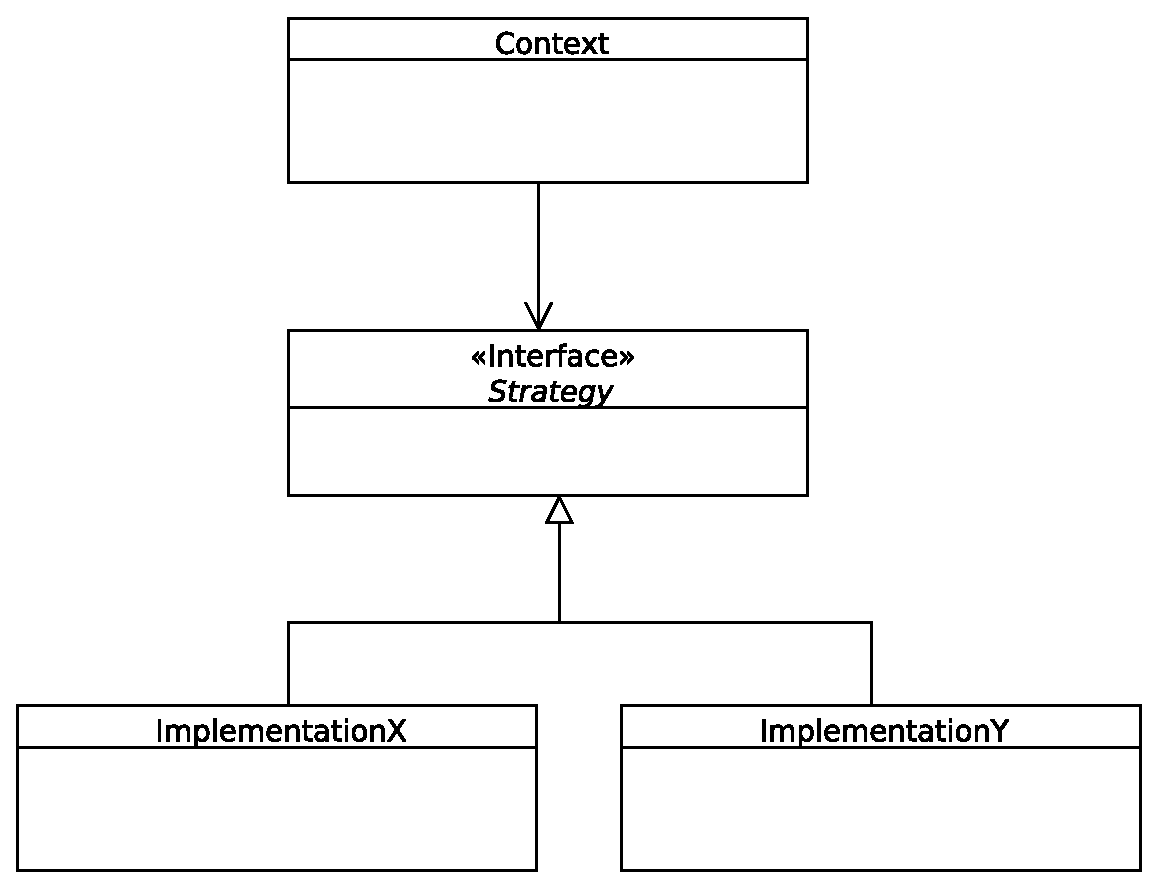
\includegraphics[width=0.6\textwidth]{strategy.eps}
\caption{Il pattern Strategy}
\label{strategy}
\end{figure}


Nel pattern Strategy, l'algoritmo è incapsulato in una classe separata rispetto al contesto in cui deve essere usato. Inoltre, tutti gli algoritmi (o meglio, tutte le classi che rappresentano un algoritmo) implementano un'interfaccia comune. L'oggetto all'interno del quale si deve adoperare un algoritmo di quel tipo avrà un riferimento all'interfaccia, rimanendo così slegata dalle classi concrete: questo rende semplice modificare in fase di manutenzione l'implementazione da utilizzare. Lo schema del pattern è raffigurato in figura \ref{strategy}; per maggiori dettagli, si consiglia \cite{gof}.\\

\subsubsection{\textsl{Filler}}

\paragraph{}
La classe che rappresenta genericamente l'algoritmo è chiamata \lstinline{ContractShareTableFiller}; per brevità, si farà di seguito riferimento ad essa con il termine \textsl{filler}. \\
Attualmente, è prevista un'unica implementazione del filler, chiamata \lstinline{StandardContractShareTableFiller} (o \textsl{filler standard}). Questa implementazione prevede tutti gli altri attributi della tabella di ripartizione vengano calcolati sulla base della quota relativa al personale. In figura \ref{filler_strategy} è mostrato il pattern Strategy applicato al caso concreto.\\
Le percentuali sulla base delle quali eseguire il calcolo sono definibili attraverso gli opportuni file di configurazione, che si trovano all'interno della sotto-cartella \path{aliquoteDipartimenti} della cartella di configurazione (path relativo alla directory di jBoss: \path{standalone/deployments/Jama.war/WEB-INF/classes/config}). \\

\begin{figure}[h]
\centering
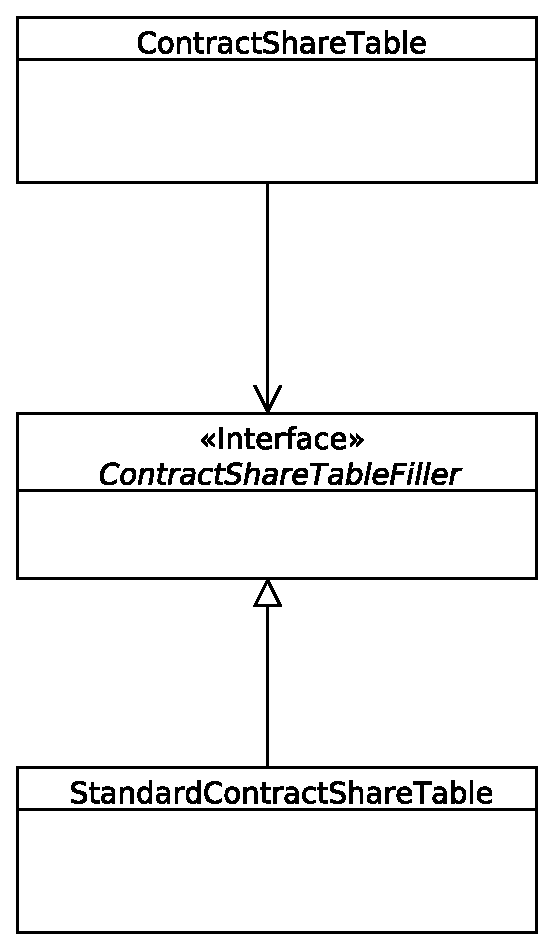
\includegraphics[width=0.25\textwidth]{filler_strategy.eps}
\caption{Il pattern Strategy applicato ai filler}
\label{filler_strategy}
\end{figure}

\paragraph{}
In realtà, in questa cartella non sono presenti file di configurazione, ma altre sotto-cartelle. Infatti, è possibile specificare aliquote diverse per ogni dipartimento, ognuno dei quali ha la propria directory, riconoscibile dall'identificativo del dipartimento stesso. Questo però ha effetti anche sul codice: non è possibile utilizzare lo stesso filler per tutti i dipartimenti. È questo il motivo per cui è stato utilizzato il pattern \textsl{Abstract factory} per incapsulare la responsabilità di istanziare il filler appropriato. Quando è necessario ottenere un filler per un dato contratto, è sufficiente chiamare il metodo \lstinline{getFiller} della factory passandogli il dipartimento del docente che lo ha stipulato. \\
Anche per la factory è necessario stabilire quale implementazione utilizzare, essendo questa legata al filler da produrre. Il meccanismo è sempre lo stesso: non si fa riferimento alla classe concreta, ma a quella di base. Se si dovesse cambiare tipo di filler, è sufficiente implementare la relativa factory ed aggiornare il resto di conseguenza. L'aggiornamento è inoltre molto più semplice nel caso della factory, perché esse non sono entità di JPA (ossia, non sono annotate \lstinline{@Entity}), ma sono bean di CDI. Questo consente di utilizzare le \textit{alternatives} (si veda il capitolo \ref{cdi} per maggiori dettagli) e quindi basta modificare il file \path{bean.xml} specificando il bean da utilizzare.\\

\paragraph{}
Le cose sono in realtà leggermente più complicate di così. Infatti, bisogna tener conto che le variazione delle quote o del metodo di calcolo stesso non devono essere retroattive. Ad esempio, se nel 2013 al Fondo Comune di Ateneo spetta il 2.5\% del totale della convenzione, mentre nel 2014 l'1\% sulla quota relativa al personale, le convenzioni stipulate nel 2013 dovranno mantenere la quota precedente (2.5\% sul totale), che siano ancora attive nel 2014 o che non lo siano. Da ciò nasce l'esigenza di aggiungere nel contratto un attributo che rappresenta il filler utilizzato e di salvare questa informazione nel database; inoltre, è necessario anche poter effettuare query sul filler stesso. Per questi motivi, nell'implementazione del pattern Strategy si è deciso di utilizzare una classe astratta invece di un'interfaccia.\\
In figura \ref{filler_complete} è mostrato lo schema completo.

\begin{figure}[h]
\centering
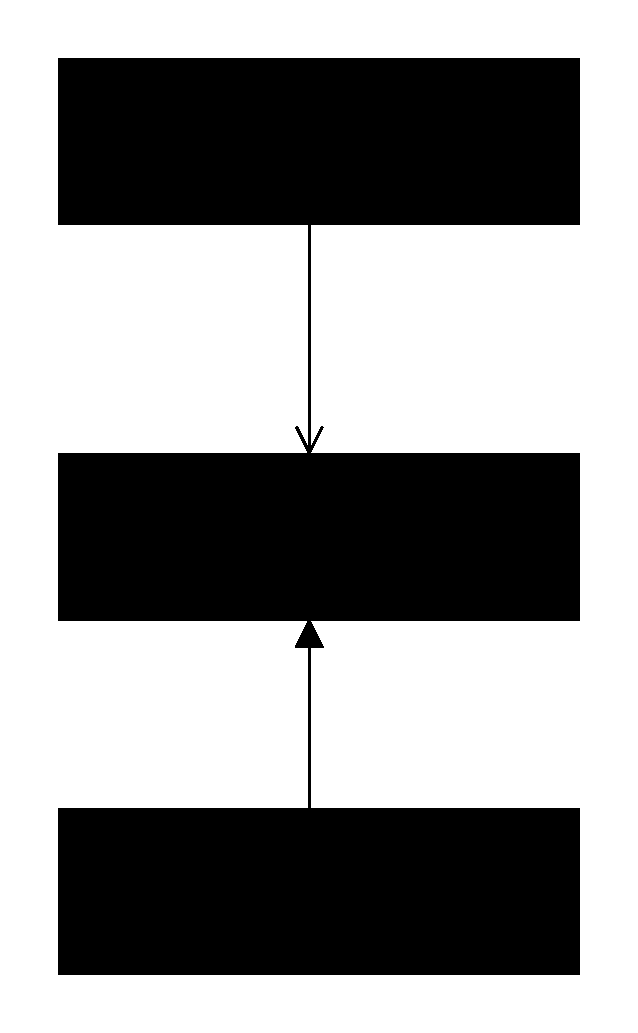
\includegraphics[width=0.6\textwidth]{filler_complete.eps}
\caption{Schema completo}
\label{filler_complete}
\end{figure}
\section{Tempo e task periodici}
Si è annoverato insieme agli agenti che interagiscono con il sistema anche il Tempo. In questa sezione si illustra come è stato realizzato questo tipo di agente, e come si sono implementate le azioni che esso compie.
In particolare si analizzano quelle azioni che possono essere classificate come task periodici e che non possono essere effettuate come conseguenza di un azione di un utente come l'Operatore, il Docente o l'Amministratore.
Un buon candidato è la notifica delle scadenze più vicine: ogni giorno ad un' ora fissata è necessario cercare le scadenze da notificare e spedire una email al docente di riferimento.

Si è scelto di rappresentare questa operazione sfruttando la classe \texttt{java.util.TimerTask}. Per definire un task occorre quindi estendere la classe \texttt{TimerTask} ed implementare il metodo \texttt{run()} come è mostrato di seguito.
\begin{lstlisting}
 
public class MyTask extends TimerTask {
	...

	@Override
	public void run() {
	
	  dostuff();

	}

}
 
\end{lstlisting}

Una volta definita l'operazione occorre schedulare la sua esecuzione impostando un tempo di partenza e un intervallo di ripetizione. Possiamo fare ciò utilizzando la classe \texttt{java.util.Timer} come mostrato di seguito.

\begin{lstlisting}
		Date date = ...;

		Timer timer = new Timer();
		TimerTask task = new MyTask();

		long interval = ...;
		timer.schedule(task, date, period);
 
\end{lstlisting}

L'ultimo problema che è necessario affrontare è come poter eseguire il codice sopra riportato all'avvio dell'\textit{application server}. La soluzione che si propone è utilizzare un bean che venga creato allo startup del server, utilizzando l'annotazione
 \texttt{@Startup}, e che contenga il codice sopra riportato in un metodo annotato con \texttt{@PostConstruct}. Un metodo così annotato verrà eseguito dopo il costruttore del bean ma prima di ogni altro metodo. Il risultato è quindi un bean così fatto:

\begin{lstlisting}
@ApplicationScoped
@Singleton
@Startup
@Named("scheduler")
public class Scheduler {

	public Scheduler() {}


	@PostConstruct
	public void schedule() {

		Date date = ...;

		Timer timer = new Timer();
		TimerTask task = new MyTask();

		long interval = ...;
		timer.schedule(task, date, period);

	}

}
\end{lstlisting}

\section{Notifiche e-mail}
Nell'applicazione ricopre un ruolo cruciale la notifica ai Docenti di ciò che riguarda contratti da lui stipulati, che avviene tramite e-mail.\\
Qui di seguito viene illustrata la struttura del codice che viene usato per questo procedimento e un esempio di template:

\begin{lstlisting}
public void notifyEvent(Contract c) {
	
	TemplateFiller filler = new TemplateFiller(c, "email@address.com");
	StringWriter out = new StringWriter();

	Template template = Config.fmconf.getTemplate(Config.templateFileName);
	temp.process(filler, out);
	String mailContent = out.toString();

	User u = userDao.getBySerialNumber(c.getChief().getSerialNumber());
	String email = u.getEmail();

	send(email, "Title", mailContent);
}

private void send(String recipientEmail, String subject, String text) {

	String host = "smtp.gmail.com";
	String username = "jama.mail.services";
	String password = "password";

	MimeMessage message = new MimeMessage(mailSession);
	try {

		message.setRecipient(RecipientType.TO, new InternetAddress(recipientEmail));
		message.setSubject(subject);
		message.setText(text);
		message.saveChanges();

		Transport t = mailSession.getTransport("smtps");
		try {
			t.connect(host, username, password);
			t.sendMessage(message, message.getAllRecipients());
		} finally {
			t.close();
		}

	} catch (MessagingException e) {
		FacesContext context = FacesContext.getCurrentInstance();
		context.addMessage(null, new FacesMessage(Messages.getString("err_sendingMail")));
	}
}

public class TemplateFiller {
	private Contract contract;
	private String mail;


	public TemplateFiller(Contract contract, String mail) {
		super();
		this.contract = contract;
		this.mail = mail;
	}


	public Contract getContract() {
		return contract;
	}


	public String getMail() {
		return mail;
	}

}
\end{lstlisting}

\begin{lstlisting}
Gent.mo Professore,
le comunichiamo che la convenzione dal titolo "${contract.title}" fra ${contract.department.name} e ${contract.company.name} e' stata chiusa, con un fatturato complessivo di ${contract.turnOver}.

Ringraziandola per l'attenzione, si inviano cordiali saluti.

Questo messaggio e' stato inviato p.c. anche al Segretario Amministrativo all'indirizzo ${mail}.
\end{lstlisting}

Come è possibile notare, viene usata la libreria FreeMarker per produrre il contenuto della mail. Si è già spiegato il suo funzionamento nel paragrafo \ref{freemarker}; qui si può vedere l'applicazione all'operazione di notifica.\\
La configurazione di FreeMarker viene definita una sola volta all'avvio, ed è accessibile tramite la classe \lstinline{util.Config} (che contiene la configurazione di Jama). La classe \lstinline{Config} espone inoltre anche gli attributi che contengono i nomi dei file di template.\\
Definita la configurazione è quindi possibile passare al caricamento del template e al suo utilizzo. Tale operazione viene eseguita nel metodo \lstinline{notifyEvent} tramite la chiamata al metodo \lstinline{getTemplate}. Quest'ultimo viene poi riempito utilizzando il bean \lstinline{TemplateFiller} e subito dopo viene prodotto l'output. \\
A questo punto viene chiamato il metodo \lstinline{send}, che è quello che si occupa dell'invio vero e proprio della posta elettronica. Per fare ciò, vengono semplicemente adoperate le API Java del package \lstinline{javax.mail}, usando gli opportuni parametri dipendenti dall'applicazione (come ad esempio l'host o il protocollo).\\
L'intero processo viene eseguito dalla classe \lstinline{MailSender}, che si trova nel package \lstinline{Util}.

\section{Valuta}
 


			

\nocite{*}		 % Mostra in bibliografia anche gli oggetti non citati 
\bibliography{biblio}{}
\bibliographystyle{plain}


\end{document}       
